\chapter{Funciones continuas}
\setcounter{section}{1}
\section{Definición de límite de una función}
La continuidad existe si existe  continuidad por la izquierda y por la derecha.

\begin{tcolorbox}
    \begin{def.}[Definición de entorno de un punto]
	Cualquier intervalo abierto que contenga un punto $p$ como su punto medio se denomina entorno de $p$.
    \end{def.}
\end{tcolorbox}

\textbf{Notación.-} Designemos los entornos con $N(p), N_1(p), N_2(p),$ etc. Puesto que un entorno $N(p)$ es un intervalo abierto simétrico respecto a $p$, consta de todos los números reales $x$ que satisfagan $p-r<x<p+r$ para un cierto $r>0$. El número positivo $r$ se llama radio del entorno. En lugar de $N(p)$ ponemos $N(p;r)$ si deseamos especificar su radio. Las desigualdades $p-r<x<p+r$ son equivalentes a $-r<x-p<r$, y a $|x-p|<r$. Así pues, $N(p;r)$ consta de todos los puntos $x$ , cuya distancia a $p$ es menor que $r$.\\
En la definición que sigue suponemos que $A$ es un número real y que $f$ es una función definida en un cierto entorno de un punto $p$ (excepción hecha acaso del mismo $p$). La función puede estar definida en $p$ pero esto no interviene en la definición.\\

\begin{tcolorbox}
    \begin{def.}[Definición de límite de una función]
	El simbolismo $$\lim_{x\to p}f(x)=A\qquad [\mbox{o}\; {f(x)\to A}\quad {x\to p}]$$
	significa que para todo entorno $N_1(A)$ existe un cierto entorno $N_2(p)$ tal que 
	\begin{center}
	    $f(x)\in N_1(A)$ siempre que $x\in N_2(p)$ y $x\neq p$
	\end{center}
	\vspace{0.3cm}
	El entorno $N_1(A)$ se cita en primer lugar, e indica cuán próximo queremos que sea $f(x)$ a su límite $A$. El segundo entorno, $N_2(p)$, nos indica lo próximo que debe estar $x$ de $p$ para que $f(x)$ sea interior al primer entorno $N_1(p)$. El entorno $N_2(p)$ dependerá del $N_1(A)$ elegido. Un entorno $N_2(p)$ que sirva para un $N_1(A)$ determinado servirá también, naturalmente, para cualquier $N_1(A)$ mayor, pero puede no ser útil para todo $N_1(A)$ más pequeño.\\
	Decir que $f(x)\in N_1(A)$ es equivalente a la desigualdad $|f(x)-A|<\epsilon$ y poner que $x\in N_2(p),\; x\neq p$ es lo mismo que escribir $0<|x-p|<\delta$. Por lo tanto, la definición de límite puede también expresarse así:\\\\
	El símbolo $\lim\limits_{x\to p}f(x)=A$ significa que para todo $\epsilon > 0$, existe un $\delta >0$ tal que $$|f(x)-A|<\epsilon \quad \mbox{siempre que}\quad 0<|x-p|<\delta.$$
    \end{def.}
\end{tcolorbox}

Observamos que las tres desigualdades,

\begin{center}
    $\lim\limits_{x\to p}f(x)=A$, $\lim\limits_{x\to p}(f(x)-A)=0$, $\lim\limits_{x\to p}[f(x)-A]=0$
\end{center}

Son equivalentes. También son equivalentes las desigualdades,
    
\begin{center}
    $\lim\limits_{x\to p} f(x)=A,$ $\lim\limits_{h\to 0}f(p+h)=A.$
\end{center}

Todas estas se derivan de la definición de límite.\\
\begin{tcolorbox}
    \begin{def.}[Límites laterales]
	Los límites laterales pueden definirse en forma parecida. Por ejemplo, si ${f(x)\to A}$ cuando ${x\to p}$ con valores mayores que $p$, decimos que $A$ es el límite por la derecha de $f$ en $p$, indicamos esto poniendo
	$$\lim_{x\to p^+}f(x)=A.$$
	En la terminología de los entornos esto significa que para todo entorno $N_1(A),$ existe algún entorno $N_2(p)$ tal que 
	$$f(x)\in N_1(A)\; \mbox{siempre que}\; x \in N_2(p)\quad \mbox{y}\quad x>p.$$
	Los límites a la izquierda, que indican poniendo ${x\to p^-}$, se definen del mismo modo restringiendo $x$ a valores menores que $p$.
    \end{def.}
\end{tcolorbox}

\section{Definición de continuidad de una función}

\begin{tcolorbox}
    \begin{def.}[Definición de continuidad de una función en un punto]
	Se dice que una función $f$ es continua en un punto $p$ si 
	\begin{enumerate}[\bfseries a)]
	    \item $f$ está definida en $p$, y
	    \item $\lim\limits_{x\to p}f(x)=f(p)$.
	\end{enumerate}
	Esta definición también puede formularse con entornos. Una función $f$ es continua en $p$ si para todo entorno $N_1[f(p)]$ existe un entorno $N_2(p)$ tal que 
	$$f(x)\in N_1[f(p)]\; \mbox{siempre que}\; x \in N_2(p).$$
	Puesto que $f(p)$ pertenece siempre a $N_1[f(p)]$, no se precisa la condición $x\neq p$.\\\\
	Especificando los radios de los entornos, la definición de continuidad puede darse como sigue:
	\begin{center}
	    $|f(x)-f(p)|<\epsilon$ siempre que $|x-p|<\delta$.
	\end{center}
    \end{def.}
\end{tcolorbox}

\section{Teoremas fundamentales sobre límites. Otros ejemplos de funciones continuas.}

%-------------------- teorema 3.1 --------------------------
\begin{tcolorbox}
    \begin{teo}
	Sean $f$ y $g$ dos funciones tales que 
	$$\lim_{x\to p} f(x)=A,\qquad \lim_{x\to p}g(x)=B$$
	Se tiene entonces
	\begin{enumerate}[\bfseries (i)]
	    \item $\lim\limits_{x\to p} [f(x)+g(x)]=A+B$,
	    \item $\lim\limits_{x\to p} [f(x)-g(x)]=A-B$,
	    \item $\lim\limits_{x\to p} f(x)\cdot g(x) = A\cdot B$,
	    \item $\lim\limits_{x\to p} \dfrac{f(x)}{g(x)} = \dfrac{A}{B}\qquad \mbox{si}\; B\neq 0$.\\
	\end{enumerate}
	Las demostraciones estarán dadas en la sección 3.5.
    \end{teo}
\end{tcolorbox}


Observemos primero que las afirmaciones del teorema pueden escribirse en forma un poco distinta. Por ejemplo, (i) puede ponerse como sigue:
$$\lim_{x\to p}[f(x)+g(x)]=\lim_{x\to p}f(x) + \lim_{x\to p}g(x).$$\\
Es costumbre indicar por $f+g$, $f-g$, $f\cdot g$ y $f/g$ las funciones cuyos valores para cada $x$ son:
$$f(x)+g(x),\quad f(x)-g(x),\quad f(x)\cdot g(x),\quad y \quad f(x)/g(x).$$\\

\begin{teo}
    Sean $f$ y $g$ dos funciones continuas en un punto $p$. La suma $f+g$, la diferencia $f-g$,  el producto $f\cdot g$ y  $g(p)\neq 0$ siempre que $g(p)\neq 0$ son también continuas en $p$.\\\\
    Demostración.-\; Puesto que $f$ y $g$ son continuas en $p$, se tiene $\lim\limits_{x\to p} f(x)=f(p)$ y $\lim\limits_{x\to p}g(x)=g(p)$. Aplicando las propiedades para límites, dadas en el teorema 3.1, cuando $A=f(p)$ y $B=g(p)$, se deduce el teorema 3.2.\\\\
\end{teo}

El teorema que sigue demuestra que si una función $g$ está intercalada entre otras dos funciones que tienen el mismo límite cuando $x\to p,$ $g$ tiene también este límite cuando $x\to p.$\\\\

% -------------------- teorema 3.3 --------------------------
\begin{teo}[Principio de intercalación]
    Supongamos que $f(x)\leq g(x)\leq h(x)$ para todo $x\neq p$ en un cierto entorno $N(p)$. Supongamos también que 
    $$\lim_{x\to p}f(x)=\lim_{x\to p}h(x)=a.$$
    Se tiene entonces $\lim_{x\to p}g(x)=a.$\\\\
	Demostración.-\; Sean $G(x)=g(x)-f(x)$, y $H(x)=h(x)-f(x)$. Las desigualdades $f\leq g\leq h$ implican $0\leq g-f\leq h-f$ o
	$$0\leq G(x)\leq H(x)$$
	para todo $x\neq p$ en $N(p)$. Para demostrar el teorema, basta probar que $G(x)\to 0$ cuando $x\to p$, dado que $H(x)\to 0$ cuando $x\to p$.\\
	Sea $N_1(0)$ un entorno cualquier de $0$. Puesto que $H(x)\to 0$ cuando $x\to p,$ existe un entorno $N_2(p)$ tal que 
	\begin{center}
	    $H(x) \in N_1(0)$ siempre que $x\in N_2(p)$ y $x\neq p.$
	\end{center}
	    Podemos suponer que $N_2(p) \subseteq N(p)$. Entonces la desigualdad $0\leq G \leq H$ establece que $G(x)$ no está más lejos de $0$ si $x$ está en $N_2(p), x\neq p$. Por consiguiente $G(x)\in N_1(0)$ para tal valor $x$ y por tanto $G(x)\to 0$ cuando $x\to p$. La misma demostración es válida si todos los límites son límites a un lado.\\\\
\end{teo}

% -------------------- teorema 3.4 --------------------------
\begin{teo}[Continuidad de las integrales indefinidas]
    Supongamos que $f$ es integrable en $[a,x]$ para todo $x$ en $[a,b]$, y sea
    $$A(x)=\int_a^x f(t)\; dt$$
    Entonces la integral indefinida $A$ es continua en cada punto de $[a,b]$ (En los extremos del intervalo tenemos continuidad a un lado.)\\\\
	Demostración.-\; Elijamos $p$ en $[a,b]$. Hay que demostrar que $A(x)\to A(p)$ cuando $x\to p.$ Tenemos
	$$A(x)-A(p)=\int_p^x f(t)\; dt$$
	Puesto que $f$ está acotada en $[a,b]$, existe una constante $M>0$ tal que $-M\leq f(t)\leq M$ para $t$ en $[a,b]$. Si $x>p$, integramos esas desigualdades en el intervalo $[p,x]$ obteniendo
	$$\int_p^x -M \;dt \leq \int_p^x f(t)\; dt\leq \int_p^x M \; dt \quad \Longrightarrow \quad -M(x-p)\leq A(x)-A(p)\leq M(x-p).$$
	Si $x<p$, obtenemos las mismas desigualdades con $x-p$ sustituida por $p-x$. Por consiguiente, en uno u otro caso podemos hacer que $x\to p$ y aplicar el principio de intercalación encontrando que $A(x)\to A(p)$. Esto prueba el teorema. Si $p$ es un extremo de $[a,b]$, tenemos que hacer que $x\to p$ desde el interior del intervalo, con lo que los límites son a un lado.
\end{teo}


\section{Demostraciones de los teoremas fundamentales sobre límites}

Demostración de (i) y (ii). Puesto que las dos igualdades:

\begin{center}
    $\lim\limits_{x\to p}f(x)=A\;$ y $\;\lim\limits_{x\to p}[f(x)-A]=0$
\end{center}

son completamente equivalentes, y como se tiene

$$f(x)+g(x)-(A+B) = [f(x)-A]+[g(x)-B],$$

basta demostrar las igualdades (i) y (ii) del teorema cuando los límites de $A$ y $B$ son ambos cero.\\
Supóngase pues, que $f(x)\to 0$ y $g(x)\to 0$ cuando $x\to p$. Se demostrará en primer lugar que $f(x)+g(x)\to 0$ cuando $x\to p$. Para ello se tiene que probar que para cada $\epsilon > 0$ existe un $\delta>0$ tal que 

\begin{center}
    $|f(x)+g(x)|<\epsilon\; $ siempre que $\;0<|x-p|<\delta.$
\end{center}

Sea $\epsilon$ dado. Puesto que $f(x)\to 0$ cuando $x\to p$, exista un $\delta_1>0$ tal que 

\begin{center}
    $|f(x)|<\dfrac{\epsilon}{2}\;$ siempre que $\; 0<|x-p|<\delta_1.$
\end{center}

Análogamente, puesto que $g(x)\to 0$ cuando $x\to p$ existe un $\delta_2>0$ tal que:

\begin{center}
    $|g(x)|<\dfrac{\epsilon}{2}\;$ siempre que $\; 0<|x-p|<\delta_2.$
\end{center}

Si se indica por $\delta$ el menor de los dos números $\delta_1$ y $\delta_2$, entonces, ambas igualdades últimas son válidas si $0<|x-p|<\delta$, y por tanto, en virtud de la desigualdad triangular, se tiene:

$$|f(x)+g(x)|\leq |f(x)|+|g(x)|<\dfrac{\epsilon}{2}+\dfrac{\epsilon}{2}=\epsilon$$

Esto demuestra la proposición dada que, a su vez, demuestra (i). La demostración de (ii) es completamente análoga, salvo que en el último paso se emplea la desigualdad $|f(x)-g(x)|\leq |f(x)|+|g(x)|.$\\\\

Demostración de (iii). Supóngase que se ha demostrado (iii) en el caso particular en que uno de los límites es $0$. Entonces el caso general resulta fácilmente de este caso particular, como se deduce de la siguiente igualdad:
$$f(x)g(x)-AB = f(x)[g(x)-B]+B[f(x)-A].$$
El caso particular implica que cada término del segundo miembro tienda a $0$ cuando $x\to p$ y en virtud de la propiedad (i) la suma de los dos términos tiende también a $0$. Por tanto, basta sólo probar (iii) en el caso en que uno de los límites, por ejemplo $B$, sea $0$.\\
Supóngase que $f(x)\to A$ y $g(x)\to 0$ cuando $x\to p$. Se trata de probar que $f(x)\cdot g(x)\to 0$ cuando $x\to p.$ Para ello se ha de ver que dado un número positivo $\epsilon,$ existe un $\delta>0$ tal que 
\begin{center}
$|f(x)g(x)|<\epsilon\;$ siempre que $\;0<|x-p|<\delta.$
\end{center}

Puesto que $f(x)\to A$ cuando $x\to p$, existe un $\delta_1$ tal que 

\begin{center}
    $|f(x)-A|<1\;$ siempre que $\; 0<|x-p|<\delta_1.$
\end{center}

Para tal $x$, tenemos $|f(x)-A+A|\leq |f(x)-A|+|A|<1+|A|,$ y por tanto

$$|f(x)g(x)|=|f(x)||g(x)|<(1+|A|)|g(x)|.$$

Ya que $f(x)\to 0$ cuando $x\to p$, para todo $\epsilon > 0$ existe un $\delta_2$ tal que 

\begin{center}
$|g(x)|<\dfrac{\epsilon}{1+|A|}\;$ siempre que $\; 0<|x-p|<\delta_2.$
\end{center}

Por consiguiente, si llamamos $\delta$ al menor de los dos números $\delta_1$ y $\delta_2$ entonces las dos igualdades son válidas siempre que $0<|x-p|<\delta$ y para tal valor de $x$ deducimos 

\begin{center}
$|f(x)g(x)|<\epsilon\;$ siempre que $\;0<|x-p|<\delta.$
\end{center}

Lo que completa la demostración.\\\\

Demostración de (iv). Puesto que el cociente $f(x)/g(x)$ es el producto de $f(x)/B$ por $B/g(x)$ basta demostrar que $B/g(x)\to 1$ cuando $x\to p$ y luego aplicar (iii). Sea $h(x)=g(x)/B$, por lo que $h(x)\to 1$ cuando $x\to p$, y se quiere demostrar que $1/h(x)$ cuando $x\to p$.\\
Dado $\epsilon>0,$ se trata de ver si existe un $\delta>0$ tal que
\begin{center}
$\bigg|\dfrac{1}{h(x)}\bigg|<\epsilon\;$ siempre que $\; 0<|x-p|<\delta.$
\end{center}
La diferencia se puede escribir como sigue:
$$\bigg|\dfrac{1}{h(x)}-1\bigg|=\dfrac{|h(x)-1|}{|g(x)|}.$$
Puesto que $g(x)\to 1$ cuando $x\to p$ se puede elegir un $\delta>0$ tal que ambas desigualdades:
$$|h(x)-1|<\dfrac{\delta}{2}\quad \mbox{y}\quad |h(x)-1|<\dfrac{1}{2}.$$
se satisfagan siempre que $0<|x-p|<\delta$. La segunda de estas desigualdades implica $h(x)>\dfrac{1}{2}$ y por tanto $1/|h(x)|=1/h(x)<2$ para tales valores de $x$. Empleando este resultado en junto con la primera desigualdad, obtenemos 
$$\bigg|\dfrac{1}{h(x)}-1\bigg|=\dfrac{|h(x)-1|}{|g(x)|}.$$
Esto completa la demostración de (iv).\\

\section{Ejercicios}

En los ejercicios del 1 al 10, calcular los límites y explicar cuáles han sido los teoremas utilizados en cada caso.\\\\

\begin{enumerate}[\bfseries 1.]

    %-------------------- 1.
    \item $\lim\limits_{x\to 2}\dfrac{1}{x^2}.$\\\\
	Respuesta.-\; 
	$$\lim\limits_{x\to 2}\dfrac{1}{x^2} = \dfrac{\lim\limits_{x\to 2}1}{\lim\limits_{x\to 2}x^2} = \dfrac{1}{2^2}=\dfrac{1}{4}.$$

	Esto por el teorema 3.1 inciso (iv) y por el hecho de que el límite de una constante es la misma constante.\\\\

    %-------------------- 2.
    \item $\lim\limits_{x\to 0} \dfrac{25x^3+2}{75x^7-2}$\\\\
	Respuesta.-\; 
	$$\lim\limits_{x\to 0} \dfrac{25x^3+2}{75x^7-2}=\dfrac{\lim\limits_{x\to 0}25x^3+\lim\limits_{x\to 0}2}{\lim\limits_{x\to 0}75x^7-\lim\limits_{x\to 0}2} = \dfrac{0 + 2}{0-2}=-1.$$
	Por el teorema 3.1 incisos (i),(ii) y (iii).\\\\

    %-------------------- 3.
    \item $\lim\limits_{x\to 2}\dfrac{x^2-4}{x-2}$.\\\\
	Respuesta.-\; 
	$$\lim\limits_{x\to 2}\dfrac{x^2-4}{x-2} = \lim_{x\to 2}\dfrac{(x-2)(x+2)}{x-2}=\lim_{x\to 2}(x+2) = \lim_{x\to 2} x + \lim_{x\to 2}2 = 4.$$
	Esto por el teorema 3.1 inciso (1).\\\\

    %-------------------- 4.
    \item $\lim\limits_{x\to 1}\dfrac{2x^2-3x+1}{x-1}$.\\\\
	Respuesta.-\; 
	$$\lim\limits_{x\to 1}\dfrac{2x^2-3x+1}{x-1} = \lim_{x\to 1}\dfrac{(2x-1)(x-1)}{x-1}=\lim_{x\to 1} 2x - \lim_{x\to 1} 1 = 1.$$
	Esto por el teorema 3.1 inciso (1).\\\\

    %-------------------- 5.
    \item $\lim\limits_{h\to 0}\dfrac{(t+h)^2-t^2}{h}.$\\\\
	Respuesta.-\; 
	$$\lim\limits_{h\to 0}\dfrac{(t+h)^2-t^2}{h} = \lim_{h\to 0}\dfrac{t^2+2th+h^2-t^2}{h}=\lim_{h \to 0} (2t+h) = \lim_{h\to 0}2t + \lim_{h\to 0}h = 2t.$$
	Esto por el teorema 3.1 inciso (1).\\\\

    %-------------------- 6.
    \item $\lim\limits_{x\to 0}\dfrac{x^2-a^2}{x^2+2ax+a^2},\qquad a\neq 0$.\\\\
	Respuesta.-\; 
	$$\lim\limits_{x\to 0}\dfrac{x^2-a^2}{x^2+2ax+a^2} = \lim_{x\to 0}\dfrac{(x-a)(x+a)}{(x+a)^2}=\lim_{x\to 0}\dfrac{x-a}{x+a}=\dfrac{\lim\limits_{x\to 0}x-\lim\limits_{x\to 0}a}{\lim\limits_{x\to 0}x + \lim\limits_{x\to 0}a} = -1.$$
	Por el teorema 3.1 incisos (i),(ii) y (iii).\\\\

    %-------------------- 7.
    \item $\lim\limits_{a\to 0}\dfrac{x^2-a^2}{x^2+2ax+a^2},\qquad a\neq 0.$\\\\
	Respuesta.-\; 
	$$\lim\limits_{a\to 0}\dfrac{x^2-a^2}{x^2+2ax+a^2} = \lim_{a\to 0}\dfrac{(x-a)(x+a)}{(x+a)^2}=\lim_{a\to 0}\dfrac{x-a}{x+a}=\dfrac{\lim\limits_{a\to 0}x-\lim\limits_{a\to 0}a}{\lim\limits_{a\to 0}x + \lim\limits_{a\to 0}a} = 1.$$
	Por el teorema 3.1 incisos (i),(ii) y (iii).\\\\

    %-------------------- 8.
    \item $\lim\limits_{x\to a}\dfrac{x^2-a^2}{x^2+2ax+a^2},\qquad a\neq 0.$\\\\
	Respuesta.-\; 
	$$\lim\limits_{x\to a}\dfrac{x^2-a^2}{x^2+2ax+a^2} = \lim_{x\to a}\dfrac{(x-a)(x+a)}{(x+a)^2}=\lim_{x\to a}\dfrac{x-a}{x+a}=\dfrac{\lim\limits_{x\to a}x-\lim\limits_{x\to a}a}{\lim\limits_{x\to a}x + \lim\limits_{x\to a}a} = 0$$
	Por el teorema 3.1 incisos (i),(ii) y (iii).\\\\

    %-------------------- 9.
    \item $\lim\limits_{t\to 0} \tan t.$\\\\
	Respuesta.-\; 
	$$\lim\limits_{t\to 0} \tan t = 0.$$\\

    %-------------------- 10.
    \item $\lim\limits_{t\to 0}(\sen 2t + t^2 \cos 5t).$\\\\
	Respuesta.-\; 
	$$\lim\limits_{t\to 0}(\sen 2t + t^2 \cos 5t) = \lim_{t\to 0}\sen 2t + \lim_{t\to 0}t^2\cdot \lim_{t\to 0}\cos 5t = 0.$$
	Por el teorema 3.1 incisos (i) y (iii).\\\\

    %-------------------- 11.
    \item $\lim\limits_{x\to 0^+}\dfrac{|x|}{x}.$\\\\
	Respuesta.-\; Ya que $|x|=x$ para $x>0$, por lo tanto tenemos  
	$$\lim_{x\to 0^+}\dfrac{|x|}{x}=\lim_{x\to 0^+}\dfrac{x}{x}=1.$$\\

    %-------------------- 12.
    \item $\lim\limits_{x\to 0^-}\dfrac{|x|}{x}.$\\\\
	Respuesta.-\; Ya que $|x|=-x$ para $x<0$, por lo tanto tenemos  
	$$\lim_{x\to 0^-}\dfrac{|x|}{x}=\lim_{x\to 0^-}\dfrac{-x}{x}=-1.$$\\

    %-------------------- 13.
    \item $\lim\limits_{x\to 0^+}\dfrac{\sqrt{x^2}}{x}.$\\\\
	Respuesta.-\; Para $x>0$ tenemos $\sqrt{x^2}=|x|=x$ entonces,
	$$\lim_{x\to 0^+}\dfrac{\sqrt{x^2}}{x}=\lim_{x\to 0^+} \dfrac{x}{x}=1.$$\\

    %-------------------- 14.
    \item $\lim\limits_{x\to 0^-}\dfrac{\sqrt{x^2}}{x}.$\\\\
	Respuesta.-\; Para $x<0$ tenemos $\sqrt{x^2}=|x|=-x$ entonces,
	$$\lim_{x\to 0^-}\dfrac{\sqrt{x^2}}{x}=\lim_{x\to 0^-} \dfrac{-x}{x}=-1.$$\\

	Utilizar la relación $\lim\limits_{x\to 0}(\sen x)/x$ para establecer las igualdades de los Ejercicios del 15 al 20.\\\\

    %-------------------- 15.
    \item $\lim\limits_{x\to 0}\dfrac{\sen 2x}{x}=2.$\\\\
	Respuesta.-\; Sea $\sen(2x) = 2\sen x \cos x$ entonces 
	$$\dfrac{\sen 2x}{x} = \dfrac{2\sen x \cos x}{x} = 2\cos x\left(\dfrac{\sen x}{x}\right)$$
	de donde 
	$$\lim_{x\to 0}\dfrac{\sen 2x}{x}=\lim_{x\to 0}\left(2\cos x \dfrac{\sen x}{x}\right) = \lim_{x\to 0}2\cdot \lim_{x\to 0}\cos x \cdot \lim_{x\to 0}\dfrac{\sen x}{x} = 2.$$\\

    %-------------------- 16.
    \item $\lim\limits_{x\to 0}\dfrac{\tan 2x}{\sen x}=2.$\\\\
	Respuesta.-\; Ya que $\tan2x = \dfrac{\sen 2x}{\cos 2x}$ entonces,
	$$\lim_{x\to 0}\dfrac{\tan 2x}{\sen x} = \lim_{x\to 0} \dfrac{\sen 2x}{\cos 2x \sen x} = \lim_{x\to 0} \dfrac{2\sen x \cos x}{\cos 2x \sen x}=\lim_{x\to 0} \dfrac{2\cos x}{\cos 2x}=2.$$\\

    %-------------------- 17.
    \item $\lim\limits_{x\to 0}\dfrac{\sen 5x}{\sen x}=5.$\\\\
	Respuesta.-\; Primeramente tenemos,
	$$\lim_{x\to 0}\dfrac{\sen 5x}{\sen x}=\lim_{x\to 0}\left[\left(\dfrac{\sen x}{x}\right)\left(\dfrac{\sen 5x}{\sen x}\right)\right]=\lim_{x\to 0}\dfrac{\sen 5x}{x}.$$
	Luego usando la formula $\sen(x+y)=\sen x \cos y + \cos x \sen y$ obtenemos,
	$$\begin{array}{rcl}
	    \lim\limits_{x\to 0}\dfrac{\sen 5x}{x}&=&\lim\limits_{x\to 0}\dfrac{\sen(4x+x)}{x}\\\\
						  &=&\lim\limits_{x\to 0}\dfrac{\sen 4x \cos x + \sen x \cos 4x}{x}\\\\
						  &=&\lim\limits_{x\to 0}\left(\dfrac{2\sen 2x \cos 2x \cos x}{x}+\dfrac{\sen x}{x}\cos 4x\right)\\\\
						  &=&\lim\limits_{x\to 0}\left(\dfrac{\sen 2x}{x}2\cos 2x \cos x + \dfrac{\sen x}{x}\cos 4x\right)\\\\
	\end{array}$$
	pero sabemos que $\lim\limits_{x\to 0}\dfrac{\sen 2x}{x}=2$, así 
	$$\lim_{x\to 0}\dfrac{\sen 5x}{\sen x}=\lim\limits_{x\to 0}\left(\dfrac{\sen 2x}{x}2\cos 2x \cos x + \dfrac{\sen x}{x}\cos 4x\right)=2\cdot 2 + 1\cdot 1 = 5.$$\\\\

    %-------------------- 18.
    \item $\lim\limits_{x\to 0}\dfrac{\sen 5x - \sen 3x}{x}=2.$\\\\
	Respuesta.-\; Sabemos por ejercicios anteriores que
	$$\lim_{x\to 0}\dfrac{\sen 5x}{x}=5,\qquad \mbox{y} \qquad \lim_{x\to 0}\dfrac{\sen 2x}{x}=2$$
	entonces 
	$$\begin{array}{rcl}
	    \lim\limits_{x\to 0}\dfrac{\sen 3x}{x}&=&\lim\limits_{x\to 0} \dfrac{\sen (2x+x)}{x}\\\\
						  &=&\lim\limits_{x\to 0}\dfrac{\sen 2x \cos x + \sen x \cos 2x}{x}\\\\
						  &=&\lim\limits_{x\to 0}\left(\dfrac{\sen 2x}{x}\cos x + \dfrac{\sen x}{x}\cos 2x\right)\\\\
	\end{array}$$
	por lo tanto
	$$\lim_{x\to 0}\dfrac{\sen 3x}{x}=2+1=3$$
	Así, por el teorema 3.1(ii),
	$$\begin{array}{rcl}
	    \lim\limits_{x\to 0}\dfrac{\sen 5x-\sen 3x}{x}&=&\lim\limits_{x\to 0}\left(\dfrac{\sen 5x}{x}-\dfrac{\sen 3x}{x}\right)\\\\
	    &=&\lim\limits_{x\to 0}\dfrac{\sen 5x}{x}-\lim\limits_{x\to 0}\dfrac{\sen 3x}{x}\\\\
	    &=&5-3\\\\
	    &=&2.\\\\
	\end{array}$$

    %-------------------- 19.
    \item $\lim\limits_{x\to a}\dfrac{\sen x - \sen a}{x-a}=\cos a.$\\\\
	Respuesta.-\; Por el teorema 2.3 (g) sabemos que 
	$$\sen a - \sen b = 2\sen \dfrac{a-b}{2} \cos \dfrac{a+b}{2}$$
	de donde 
	$$\lim_{x\to a}\dfrac{sen x-\sen a}{x-a}=\lim_{x\to a}\dfrac{2\sen \dfrac{x-a}{2}\cos \dfrac{x+a}{2}}{x-a} = \lim_{x\to a}\left(\dfrac{\sen \dfrac{x-a}{2}}{\dfrac{x-a}{2}}\cos \dfrac{x+a}{2}\right)$$
	pero,
	$$\lim_{x\to a}\dfrac{\sen \dfrac{x-a}{2}}{\dfrac{x-a}{2}}=\lim_{y\to 0}\dfrac{\sen y}{y}=1,\qquad \mbox{ya que, } \;y=\dfrac{x-a}{2} \; \mbox{ e } \; y\to 0 \;\mbox{ como }\; x\to a.$$
	así,
	$$\lim_{x\to a}\dfrac{\dfrac{x-a}{2}}{\dfrac{x-a}{2}}\cos \dfrac{x+a}{2}=\lim_{x\to a}\dfrac{x+a}{2}=\cos a.$$


    %-------------------- 20.
    \item $\lim\limits_{x\to 0}\dfrac{1-\cos x}{x^2}=\dfrac{1}{2}.$\\\\
	Respuesta.-\; Sea,
	$$\lim_{x\to 0}\dfrac{1-\cos x}{x^2}=\lim_{x\to 0} \dfrac{(1-\cos x)(1+\cos x)}{x^2(1+\cos x)}=\lim_{x\to 0}\dfrac{1-\cos^2 x}{x^2(1+\cos x)}$$
	Luego, ya que $\cos^2x+\sen^2 x = 1 \; \Longrightarrow \; 1-\cos^2x = \sen^2x,$ entonces
	$$\begin{array}{rcl}
	    \lim\limits_{x\to 0}\dfrac{1-\cos^2 x}{x^2(1+\cos x)}&=&\lim\limits_{x\to 0}\left(\dfrac{\sen^2 x}{x}\cdot \dfrac{1}{1+\cos x}\right)\\\\
								 &=&\lim\limits_{x\to 0}\left[\left(\dfrac{\sen x}{x}\right)^2 \dfrac{1}{1+\cos x}\right]\\\\
								 &=&\lim\limits_{x\to 0}\left[\dfrac{\sen x}{x}\cdot \dfrac{\sen x}{x}\cdot \dfrac{1}{1+\cos x}\right]\\\\
								 &=&\lim\limits_{x\to 0}\dfrac{1}{1+\cos x}\\\\
								 &=&\dfrac{1}{2}.\\\\


	\end{array}$$

    %-------------------- 21.
    \item Demostrar que $\lim\limits_{x\to 0}\dfrac{1-\sqrt{1-x^2}}{x^2}=\dfrac{1}{2}.$\\\\
	Demostración.-\; Multiplicando por el límite dado por $1+\sqrt{1-x^2}$ tenemos,
	$$\begin{array}{rcl}
	    \lim\limits_{x\to 0}&=&\lim\limits_{x\to 0}\dfrac{1-(1-x^2)}{x^2(1+\sqrt{1-x^2})}\\\\
				&=&\lim\limits_{x\to 0}\dfrac{x^2}{x^2(1+\sqrt{1-x^2})}\\\\
				&=&\lim\limits_{x\to 0}\dfrac{1}{1+\sqrt{1-x^2}}\\\\
				&=&\dfrac{1}{2}\\\\\
	\end{array}$$

    %-------------------- 22.
    \item Una función $f$ está definida como sigue:
    $$f(x)=\left\{\begin{array}{rcl}
	\sen x & \mbox{si} & x\leq c,\\
	ax+b & \mbox{si} & x>c,\\
    \end{array}\right.$$
    siendo $a,b,c$ constantes. Si $b$ y $c$ están dados, hallar todos los valores de $a$ (si existe alguno) para los que $f$ es continua en el punto $x=c$.\\\\
	Respuesta.-\; Por definición de continuidad, de una función en un punto, conocemos que $f$ es continua en $x=c$ el cual significa que $f$ está definida en $c$ y $\lim\limits_{x\to c} f(x)=f(c)$.\\
	Ya que $\sen x$ y $ax+b$ son definidos para todo $x\in \mathbb{R}$, conocemos que $f$ es conocida en $x=c$ para todo $c\in \mathbb{R}$. Entonces podemos encontrar valores de $a$ tal que 
	$$\lim_{x\to c}f(x)=f(c).$$
	Por la definición de $f$, sabemos que
	$$f(c)=\sen c$$
	Entonces, evaluamos el limite en $x\to c$ a través de valores mayores que $c$ (ya que el límite en $x\to c$ a través de valores menos que $c$ es $f(c)$ ya que $\sen x$ es una función continua y para valores menores que $c,$ $f(x)=\sen x$),
	$$\lim_{x\to c^+}f(x)=\lim_{x\to c^+} ax+b=ac+b$$
	y por lo tanto, para que $f$ sea continua en $c$ debemos tener,
	$$ac+b=\sen c\; \Longrightarrow\; b=0,\; \mbox{ y } a \mbox{ es arbitrario}.$$\\

    %-------------------- 23.
    \item Resolver el ejercicio 22 si $f$ se define de este modo:
    $$f(x)=\left\{\begin{array}{rcl}
	2\sen x & \mbox{si} & x\leq c,\\
	ax^2+b & \mbox{si} & x>c,\\
    \end{array}\right.$$
	Respuesta.-\; Por la definición de continuidad, conocemos que $f$ es continua en $x=c$ el cual significa que $f(c)$ es definida y $\lim\limits_{x\to c}f(x)=f(c)$. Ya que $2\cos x$ y $ax^2+b$ está definida para todo $x\in \mathbb{R}$, conocemos que $f$ es definida para todo $c\in \mathbb{R}$. Entonces para demostrar que es continua debemos demostrar
	$$\lim_{x\to c}f(x)=f(c).$$
	De la definición de $f$ sabemos 
	$$f(c)=2\cos c.$$
	Entonces, tomando el límite como $x$ se aproxima a $c$ por la derecha (ya que $\lim\limits_{x\to c^-} f(x)=f(c)$,  $2\cos x$ es continua y $f(x)=2\cos x$ cuando $x$ se aproxima a $c$ por la izquierda),
	$$\lim_{x\to c^+}f(x)=\lim_{x\to c^+} ax^2+b=ac^2+b.$$
	Así, debemos tener
	$$ac^2+b=2\cos c \; \Longrightarrow \; a=\dfrac{2\cos -b}{c^2} \mbox{ si } c\neq 0.$$
	Si $c=0$ entonces,
	$$ac^2+b=2\cos c \; \Longrightarrow \; b=2\, \mbox{ y } a \mbox{ es arbitrario}.$$\\

    %-------------------- 24.
    \item ¿En qué punto son funciones continuas la tangente y la cotangente?.\\\\
	Respuesta.-\; Sea $$\tan x = \dfrac{\sen x}{\cos x}$$
	y $\sen x,\, \cos x$ son continuas para todo los número reales de donde sabemos por el teorema 3.2 que $\tan x$ es continua en todas partes, por lo que $\cos x$ no es cero. Probamos que 
	$$\cos x=0 \; \Longleftrightarrow \; x=\dfrac{\pi}{2}+n\pi,\quad n\in \mathbb{Z}.$$
	por lo que $\tan x$ es continuo para 
	$$\lbrace x\in \mathbb{R} | x\neq \dfrac{\pi}{2}+n\pi,\; n\in \mathbb{Z} \rbrace$$
	Similarmente 
	$$\cot x = \dfrac{\cos x}{\sen x}$$
	 y por el teorema 3.2 tenemos que $\cot x$ es continua en todo lugar donde $\sen x$ no sea cero. Luego probamos que,
	 $$\sen x = 0\; \Longleftrightarrow \; x=n\pi \quad n  \in \mathbb{Z}.$$
	 Por lo tanto, $\cot x$ es continua para 
	 $$\lbrace x\in \mathbb{R} | x\neq n\pi, \; n \in mathbb{R}\rbrace.$$\\\\

    %-------------------- 25.
    \item Sea $f(x)=(\tan x/x)$ si $x\neq 0$. Esbozar la gráfica de $f$ correspondientes a los intervalos semiabiertos $[-\frac{1}{4}\pi,0]$. ¿Qué le ocurre a $f(x)$ cuando $x\to 0$? ¿Puede definirse $f(0)$ de modo que $f$ se haga continua en $0$?.\\\\
	Respuesta.-\; 
	    \begin{center}
		\begin{tikzpicture}
		\begin{axis}[scale=.7,draw opacity = .5, style={
		  domain=-1/4*pi:0,samples=100,smooth}, 
		  axis x line=center, % no box around the plot, only x and y axis
		  axis y line=center, % the * suppresses the arrow tips
		  ylabel = {$f(x)$},
		  xlabel = {$x$},
		  xlabel style={below right},
		  ylabel style={above left},
		  xmin=-1/4*pi,xmax=0,ymin=0,ymax=1.5,
		  enlargelimits=upper] % extend the axes a bit to the right and top
		  \addplot[black,opacity=1]{tan(deg(x))/x};
		\end{axis}
	    \end{tikzpicture}
	    \end{center}
	    \vspace{.5cm}

	    Tenemos que,
	    $$\begin{array}{rcl}
		\lim\limits_{x\to 0}\dfrac{\tan x}{x}&=&\lim\limits_{x\to 0}\dfrac{\sen x}{x\cos x}\\\\
						     &=&\lim\limits_{x\to 0}\left[\left(\dfrac{\sen x}{x} \right)\cos x\right]\\\\
						     &=&\lim\limits_{x\to 0}\cos x\\\\
						     &=&1.\\\\
	    \end{array}$$
	    ya que $f(x)=\dfrac{\tan x}{x}$ no está definida en cero entonces no es una función continua. Sin embargo, dado que el límite existe, podríamos redefinir $f$ por:
	    $$f(x)=\left\{\begin{array}{rcl}
		\dfrac{\tan x}{x}&\mbox{si}&x\neq 0\\\\
		1&\mbox{si}&x = 0\\\\
	    \end{array}\right.$$
	    \vspace{.5cm}

    %-------------------- 26.
	\item Este ejercicio ofrece otra demostración de la continuidad de las funciones seno y coseno. a) La desigualdad $|\sen x|<|x|$, válida para $0<|x|<\frac{1}{2}\pi$, fue demostrada en el ejercicio 34 de la sección 2.8. Utilizarla para demostrar que la función seno es continua en $0$. b) Hacer uso de la parte a) y de la identidad $\cos 2x = 1-2\sen^2 x$ para demostrar la continuidad del coseno en $0$.\\\\
	    Demostración.-\; Demostraremos primeramente que $\lim\limits_{x\to 0}\sen x = \sen 0 = 0$.\\
	    Para todo $\epsilon>0$ existe un $\delta >0$ tal que $|\sen x|<\epsilon$ entonces $|x|<\delta$. Sea $\delta = \epsilon$, se tiene
	    $$|\sen x|<|x|\delta = \epsilon,\qquad \mbox{de donde }0<|x|<\delta$$
	    así, $\sen x$ es continua en $0$.\\
	    Por último usando la identidad dada, tenemos que
	    $$\cos(2x)=1-2\sen^2 x\; \Longrightarrow \; \cos x  1-2\sen^2\dfrac{x}{2},$$
	    por lo tanto
	    $$\begin{array}{rcl}
		\lim\limits_{x\to 0}\cos x&=&\lim\limits_{x\to 0}\left(1-2\sen^2\dfrac{x}{2}\right)\\\\
					  &=&1-2\lim\limits_{x\to 0}\left[\sen\left(\dfrac{x}{2}\right)\sen \left(\sen \dfrac{2}{x}\right)\right]\\\\
					  &=&1\\\\
					  &=&\cos 0.
	    \end{array}$$
	    así, el coseno es continuo en $0$.\\\\

    %-------------------- 27.
    \item La figura siguiente muestra una proporción de la gráfica de la función $f$ definida como sigue:
	$$f(x)=\sen \dfrac{1}{x}\quad \mbox{si}\quad x\neq 0$$
	Para $x=1/(n\pi)$, siendo $n$ entero, tenemos $\sen(1/x)=\sen(n\pi)=0$. Entre dos de esos puntos, la función asciende hasta $1$ y baja otra vez hasta $0$ o bien desciende a $-1$ y vuelve a subir a $0$. Por consiguiente, entre cualquiera de esos puntos y el origen, la curva presenta infinitas oscilaciones. Esto sugiere que los valores de la función no tienden a ningún valor fijo cuando $x\to 0$. Demostrar que no existe ningún valor real $A$ tal que $f(x)\to A$ cuando $x\to 0.$ Esto demuestra que no es posible definir $f(0)$ de manera que $f$ sea continua en $0$.\\
	    \begin{center}
		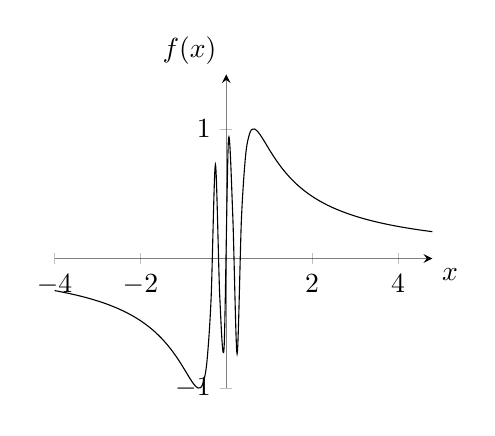
\begin{tikzpicture}
		\begin{axis}[scale=.7,draw opacity =.5,samples=100,smooth, 
		  axis x line=center, % no box around the plot, only x and y axis
		  axis y line=center, % the * suppresses the arrow tips
		  ylabel = {$f(x)$},
		  xlabel = {$x$},
		  xlabel style={below right},
		  ylabel style={above left},
		  xmin=-4,xmax=4,ymin=-1,ymax=1.2,
		  enlargelimits=upper] % extend the axes a bit to the right and top
		  \addplot[black,opacity=1]{sin(deg(1/x))};
		\end{axis}
	    \end{tikzpicture}
	    \end{center}
	    \vspace{.5cm}

	    Demostración.-\; Supongamos que existe algún $A\in \mathbb{R}$ tal que $\lim\limits_{x\to 0}f(x)=A.$ De la definición de límites esto significa que para todo $\epsilon>0$ existe un $\delta>0$ tal que 
	    $$|f(x)-A|<\epsilon\; \mbox{siempre que}\; 0<|x|<\delta$$
	    Primero, afirmamos que para cualquiera de estos $A$ debemos tener $|A|\leq 1$. Debe ser así porque si $|A|>1$ entonces $|A|-1>0$, de donde podríamos elegir $\epsilon$ tal que $0<\epsilon<(|A|-1)$. Pero se tiene $|f(x)|\leq 1$ para todo $x$, por consiguiente
	    $$|f(x)-A|=|A-f(x)|\geq |A|-|f(x)|\geq |A|-1>\epsilon$$
	    Esto contradice nuestra elección de $\epsilon$, por lo que $|A|$ deber ser menor o igual que 1.\\
	    Luego supongamos $|A|\leq 1$ y elegimos $\epsilon=\frac{1}{2}>0$. Para obtener nuestra contradicción debemos demostrar que no existe $\delta > 0$ tal que
	    $$|f(x)-A|<\dfrac{1}{2}\; \mbox{ siempre que } 0<|x|<\delta$$
	    Por la propiedad de Arquímedes de los números reales sabemos que para cualquier $x\in \mathbb{R}$, existe un entero positivo tal que $n$ con $n=1\; (modk\; 4)$. Pero,
	    $$0<\dfrac{2}{n\pi}<|x|\; \Longrightarrow \; 0<\dfrac{2}{(n+2)\pi}<|x|$$
	    Entonces, por la definición de $f$ y ya que $n=1\; (mod \;4)$ y $n+2=3\; (\mod\; 4)$, tenemos 
	    $$f\left(\dfrac{2}{n\pi}\right)=\sen\left(\dfrac{n\pi}{2}\right)=1 \qquad \quad f\left[\dfrac{2}{(n+2)\pi}\right]=\sen\left[\dfrac{(n+2)\pi}{2}\right]=-1$$
	    pero,
	    $$\bigg|f\left(\dfrac{n\pi}{2}\right)-A\bigg|\; \Longrightarrow \; |1-A|<\dfrac{1}{2} \; \Longrightarrow\; \dfrac{1}{2}<A\leq 1$$
	    Además,
	    $$\bigg|f\left[\dfrac{(n+2)\pi}{2}\right]-A\bigg|=|-1-A|>\dfrac{1}{2}.$$
	    Esto contradice que si $\lim\limits_{x\to 0}f(x)=A$ entonces para cada $\epsilon>0$ tenemos $|f(x)-A|<\epsilon$ para todo $0<|x|<\delta$. En otras palabras, encontramos un $\epsilon$ mayor que $0$ tal que no importa tan pequeño que elijamos $\delta$ existe un $x$ tal que $|x|$ es menor que $\delta$, pero $|f(x)-A|$ es mayor que $\epsilon$. Esto contradice la definición de $\lim\limits_{x\to 0}f(x)=A$. Por lo tanto no puede haber tal núemero en $A\in \mathbb{R}$.\\\\

    %-------------------- 28.
    \item Para $x\neq 0$, sea $f(x)=[1/x]$, designado por $[t]$ el mayor entero $\leq t.$ Trazar la gráfica de $f$ para los intervalos $[-2,-\frac{1}{5}]$ y $[\frac{1}{5},2]$. ¿Qué le ocurre a $f(x)$ cuando $x\to 0$ tomando valores positivos? ¿y tomando valores negativos? ¿Puede definirse $f(0)$ para que $f$ sea continuo en $0$? \\\\
	Respuesta.-\; 
	\begin{center}
	    \begin{tikzpicture}
	    \begin{axis}[scale=1.2,draw opacity =.5,samples=100,smooth, 
	      axis x line=center, 
	      axis y line=center,
	      ylabel = {$f(x)$},
	      xlabel = {$x$},
	      xlabel style={below right},
	      ylabel style={above left},
	      xmin=-2,xmax=2,ymin=-5,ymax=4,
	      label style={font=\tiny},
	      tick label style={font=\tiny},
	      enlargelimits=upper] 
	      \addplot[black,opacity=1,domain=-2:-1]{-1};
	      \addplot[fill=white,mark=*] coordinates {(-2,-1)};
	      \addplot[mark=*] coordinates {(-1,-1)};
	      \addplot[black,opacity=1,domain=-1:-.5]{-2};
	      \addplot[fill=white,mark=*] coordinates {(-1,-2)};
	      \addplot[mark=*] coordinates {(-.5,-2)};
	      \addplot[black,opacity=1,domain=-.5:-.35]{-3};
	      \addplot[fill=white,mark=*] coordinates {(-.5,-3)};
	      \addplot[mark=*] coordinates {(-.35,-3)};
	      \addplot[black,opacity=1,domain=-.35:-.25]{-4};
	      \addplot[fill=white,mark=*] coordinates {(-.35,-4)};
	      \addplot[mark=*] coordinates {(-.25,-4)};
	      \addplot[black,opacity=1,domain=-.25:-.15]{-5};
	      \addplot[fill=white,mark=*] coordinates {(-.25,-5)};
	      \addplot[mark=*] coordinates {(-.15,-5)};
	      \addplot[black,opacity=1,domain=.20:.25]{4};
	      \addplot[fill=white,mark=*] coordinates {(.2,4)};
	      \addplot[mark=*] coordinates {(.25,4)};
	      \addplot[black,opacity=1,domain=.25:.35]{3};
	      \addplot[fill=white,mark=*] coordinates {(.25,3)};
	      \addplot[mark=*] coordinates {(.35,3)};
	      \addplot[black,opacity=1,domain=.35:.5]{2};
	      \addplot[fill=white,mark=*] coordinates {(.35,2)};
	      \addplot[mark=*] coordinates {(.5,2)};
	      \addplot[black,opacity=1,domain=.5:1]{1};
	      \addplot[fill=white,mark=*] coordinates {(.5,1)};
	      \addplot[mark=*] coordinates {(1,1)};
	      \addplot[black,opacity=1,domain=1:2]{0};
	      \addplot[fill=white,mark=*] coordinates {(1,0)};
	      \addplot[mark=*] coordinates {(2,0)};
	    \end{axis}
	\end{tikzpicture}
	\end{center}
	\vspace{.5cm}
	Como $x\to 0^+,\; f(x)$ toma valores positivos arbitrariamente grandes.\\
	Como $x\to 0^-,\; f(x)$ toma valores negativos arbitrariamente grandes.\\
	No hay manera de definir $f(0)$ para que $f$ sea continuo en $0$.\\\\

    %-------------------- 29.
    \item Hacer lo mismo que en el ejercicio 28, cuando $f(x)=(-1)^{[1/x]}$ para $x\neq 0$.\\\\
	Respuesta.-\;
	\begin{center}
	    \begin{tikzpicture}
	    \begin{axis}[scale=1.2,draw opacity =.5,samples=100,smooth, 
	      axis x line=center, 
	      axis y line=center,
	      ylabel = {$f(x)$},
	      xlabel = {$x$},
	      xlabel style={below right},
	      ylabel style={above left},
	      xmin=-2,xmax=2,ymin=-1.5,ymax=1.5,
	      label style={font=\tiny},
	      tick label style={font=\tiny},
	      enlargelimits=upper] 
	      \addplot[black,opacity=1,domain=-2:-1]{-1};
	      \addplot[black,opacity=1,domain=-1:-.5]{1};
	      \addplot[black,opacity=1,domain=-.5:-.3]{-1};
	      \addplot[black,opacity=1,domain=-.3:-.23]{1};
	      \addplot[black,opacity=1,domain=-.23:-.2]{-1};

	      \addplot[black,opacity=1,domain=.2:.23]{1};
	      \addplot[black,opacity=1,domain=.23:.3]{-1};
	      \addplot[black,opacity=1,domain=.3:.5]{1};
	      \addplot[black,opacity=1,domain=.5:1]{-1};
	      \addplot[black,opacity=1,domain=1:2]{1};
	    \end{axis}
	\end{tikzpicture}
	\end{center}
	\vspace{.5cm}
	Como $x\to 0^+,\; f(x)$ alterna entre $1$ y $-1$.\\
	Como $x\to 0^-,\; f(x)$ alterna entre $1$ y $-1$.\\
	No hay forma  de definir $f(0)$ para que $f$ sea continuo en $0$, ya que $f(x)$ tomará ambos valores $1$ y $-1$ no importa cuán pequeño elijamos nuestro $\delta>0$.\\\\

    %-------------------- 30.
    \item Los mismo que en el ejercicio 28, cuando $f(x)=x(-1)^{[1/x]}$ para $x\neq 0$.\\\\
	Respuesta.-\;
	\begin{center}
	    \begin{tikzpicture}
	    \begin{axis}[scale=1,draw opacity =.5,samples=100,smooth, 
	      axis x line=center, 
	      axis y line=center,
	      ylabel = {$f(x)$},
	      xlabel = {$x$},
	      xlabel style={below right},
	      ylabel style={above left},
	      xmin=-2,xmax=2,ymin=-1.5,ymax=1.5,
	      label style={font=\tiny},
	      tick label style={font=\tiny},
	      enlargelimits=upper] 
	      \addplot[black,opacity=1,domain=-2:-1]{-x};
	      \addplot[black,opacity=1,domain=-1:-.5]{x};
	      \addplot[black,opacity=1,domain=-.5:-.37]{-x};
	      \addplot[black,opacity=1,domain=-.37:-.3]{x};
	      \addplot[black,opacity=1,domain=-.3:-.25]{-x};
	      \addplot[black,opacity=1,domain=.25:.3]{x};
	      \addplot[black,opacity=1,domain=.3:.37]{-x};
	      \addplot[black,opacity=1,domain=.37:.5]{x};
	      \addplot[black,opacity=1,domain=.5:1]{-x};
	      \addplot[black,opacity=1,domain=1:2]{x};
	    \end{axis}
	\end{tikzpicture}
	\end{center}
	\vspace{.5cm}
	Como $x\to 0^+$, $f(x)\to 0$.\\
	Como $x\to 0^-$, $f(x)\to 0$.\\
	Si definimos $f(0)=0$ entonces $f$ es continuo en $0$.\\\\

    %-------------------- 31.
    \item Dar un ejemplo de una función continua en un punto de un intervalo y discontinua en los demás puntos del intervalo, o probar que no existe una tal función.\\\\
	Demostración.-\; Sea $f$ una función en el intrevalo $[-a,a]$ tal que,
	$$f(x)=\left\{\begin{array}{rcl}
		x & \mbox{para} & x\in \mathbb{Q}\\
		-x & \mbox{para} & x\in \mathbb{R}\\
	\end{array}\right.$$
	Por lo tanto, la función $f$ es continua solo en el punto $x=0$, y discontinuo en todos los demás puntos del intervalo $[-a,a]$.\\\\

    %-------------------- 32.
    \item Sea $f(x)=x\sen (1/x)$ si $x\neq 0$. Definir $f(0)$ de manera que $f$ sea continua en $0$.\\\\
	Demostración.-\; Ya que $-1\leq \sen \dfrac{1}{x}\leq 1$ para todo $x\neq 0$ sabemos que,
	$$-x\leq x\sen\dfrac{1}{x}\leq x,\quad x\neq 0$$
	después se tiene que,
	$$\lim_{x\to 0}-x=\lim_{x\to 0}x=0$$
	Aplicando el teorema 3.3 concluimos,
	$$\lim_{x\to 0}x\sen\dfrac{1}{x}=0$$
	Por lo tanto, definiendo $f(0)=0$, extendemos $f$ a una función continua en $0$.\\\\

    %-------------------- 33.
    \item Sea $f$ una función tal que $|f(u)-f(v)|\leq |u-v|$ para todos los valores $u$ y $v$ de un intervalo $[a,b]$.

	    \begin{center}
		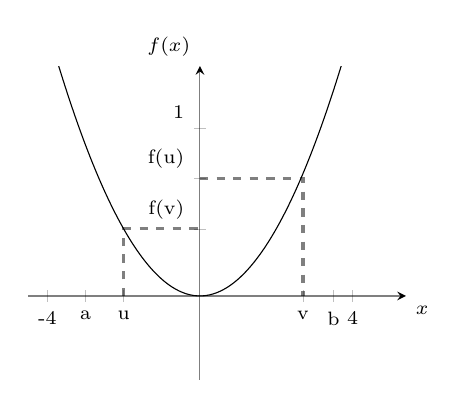
\begin{tikzpicture}
		\begin{axis}[scale=.7,draw opacity =.5,samples=100,smooth, 
		  axis x line=center, % no box around the plot, only x and y axis
		  axis y line=center, % the * suppresses the arrow tips
		  ylabel = {$f(x)$},
		  xlabel = {$x$},
		  xlabel style={below right},
		  ylabel style={above left},
		  label style={font=\scriptsize},
	          tick label style={font=\scriptsize},
		  yticklabel style={above left},
		  xtick={-4,-3,-2,2.7,3.5,4},
		  xticklabels={-4,a,u,v,b,4},
		  ytick={.7,.4,1},
		  yticklabels={f(u),f(v),1},
		  xmin=-4.5,xmax=4.5,ymin=-.5,ymax=1.2,
		  enlargelimits=upper] % extend the axes a bit to the right and top
		  \addplot[black,opacity=1]{x^2/10};
		  \addplot+[
		    black,very thick,dashed,
		    mark=none,
		    const plot,
		    empty line=jump,
		    ]
		    coordinates{
			(-2,0)
			(-2,.4)
			(0,.4)

			(0,.7)
			(2.7,.7)
			(2.7,0)
		    };
		\end{axis}
	    \end{tikzpicture}
	    \end{center}
	    \vspace{.5cm}

	\begin{enumerate}[\bfseries a)]

	    %---------- a)
	    \item Probar que $f$ es continua en cada punto de $[a,b]$.\\\\
		Demostración.-\; Sea $h$ cualquier punto en $[a,b]$, de donde para todo $\epsilon>0$ con $\delta=\epsilon$ se tiene por hipótesis que,
		$$|x-h|<\delta \;  \Longrightarrow \; |x-h|<\epsilon \; \Longrightarrow \; |f(x)-f(h)|<\epsilon$$
		Así, para todo $\epsilon>0$, tenemos $|f(x)-f(h)|<\epsilon$ siempre que $|x-h|<\delta$, y por lo tanto
		$$\lim_{x\to h}f(x)=f(h).$$\\\\


	    %---------- b)
	    \item Suponiendo que $f$ sea integrable en $[a,b]$, demostrar que
		$$\bigg|\int_a^b f(x)\; dx - (b-a)f(a)\bigg|\leq \dfrac{(b-a)^2}{2}$$
		Demostración.-\; Sea $x\in [a,b]$ tenemos,
		$$|f(x)-f(a)|\leq |x-a|=x-a$$
		y sabemos que,
		$$\int_a^b f(a)\; dx = (b-a)f(a)$$
		entonces,
		$$\begin{array}{rcl}
		    \bigg|\displaystyle\int_a^b f(x)\; dx - (b-a)f(a)\bigg|&=&\bigg|\displaystyle\int_a^b f(x)\; dx - \displaystyle\int_a^b f(a)\; dx\bigg|\\\\
									   &=&\bigg|\displaystyle\int_a^b \left[f(x)-f(a)\right]\; dx\bigg|\\\\
					 &\leq &\displaystyle\int_a^b|f(x)-f(a)|\; dx\\\\
					 &\leq &\displaystyle\int_a^b |x-a|\; dx = \int_a^b (x-a)\;dx\\\\
					 &=&\dfrac{x^2}{2}-ax\bigg|_a^b = \dfrac{(b-a)^2}{2}\\\\
		\end{array}$$
		\vspace{.5cm}

	    %---------- c)
	    \item Más general. Demostrar que para cualquier $c$ de $[a,b]$, se tiene
		$$\bigg|\int_a^b f(x)\; dx - (b-a)f(c)\bigg|\leq \dfrac{(b-a)^2}{2}$$
		Demostración.-\; Similar a la parte (b) se tiene que,
		$$\begin{array}{rcl}
		    \bigg|\displaystyle\int_a^b f(x)\; dx - (b-a)f(c)\bigg|&=&\bigg|\displaystyle\int_a^b f(x)\; dx - \displaystyle\int_a^b f(c)\; dx\bigg|\\\\
									   &\leq &\displaystyle\int_a^b|f(x)-f(c)|\; dx\\\\
									   &=&\displaystyle\int_a^b |x-c|\; dx\\\\
		\end{array}$$
		Luego ya que $c\in [a,b]$ y $|x-a|=-(x-c)$ para $x<c$ y $|x-c|=x-c$ para $x\geq c$,
		$$\begin{array}{rcl}
		    \displaystyle\int_a^b|x-c|\; dx&=&\displaystyle\int_a^c -(x-c)\; dx + \int_c^b (x-c)\; dx\\\\
						   &=&-\dfrac{x^2}{2}\bigg|_a^c +c\cdot x\bigg|_a^c +\dfrac{x^2}{2}\bigg|_c^b - c\cdot x\bigg|_c^b\\\\
						   &=&\dfrac{a^2-c^2}{2}+c(c-a)+\dfrac{b^2-c^2}{2} - c(b-c)\\\\
						   &=&\dfrac{a^2+b^2}{2}+c^2-c(b+a)\\\\
		\end{array}$$
		Pero, sabemos que $c\in[a,b]$ implica que $c\leq b$ por lo que 
		$$\begin{array}{rcl}
		    \dfrac{a^2+b^2}{2}+c^2-c(b+a)&=&\dfrac{a^2+b^2}{2}+c[c-(b+a)]\\\\
		    &\leq&\dfrac{b^2+a^2}{2}+b(b-b-a)\\\\
		    &=&\dfrac{b^2+a^2}{2}-ab\\\\
		    &=&\dfrac{b^2-2ab+a^2}{2}\\\\
		    &=&\dfrac{(b-a)^2}{2}\\\\
		\end{array}$$

	\end{enumerate}

\end{enumerate}


\section{funciones compuestas y continuas}

\begin{tcolorbox}
    \begin{def.}
	Sean $u$ y $v$ dos funciones dadas cualquiera. La compuesta o la composición de $u$ y $v$ en ese orden se define como la función $f$ para la cual
	$$f(x)=u[v(x)]$$
	Es decir, para calcular el valor de $f$ en $x$ primero se calcula $v(x)$ y luego se calcula $u$ e el punto $v(x)$. Naturalmente que para que este cálculo tenga sentido, es necesario que los valores de $v(x)$ entren en el dominio de la función $u$, y $f$ estará sólo definida en aquellos puntos $x$ para los cuales $v(x)$ está en el dominio de $u$.
    \end{def.}
\end{tcolorbox}

La notación para indicar composición es: 
$$f=u\circ v$$
que tiene una analogía con la notación de producto $u\cdot v$. En efecto, se verá a continuación que la operación de composición tiene algunas de las propiedades de la multiplicación
La \textbf{ley asociativa} está dada por:
$$u\circ(v\circ w) = (u\circ v)\circ w$$
La demostración  inmediata. Luego la ley conmutativa no es siempre válida en la composición.\\

\begin{teo}
    Suponiendo que $v$ continua en $p$ y que $u$ es continua en $q$, siendo $q=v(p)$, la función compuesta $f=u\circ v$ es continua en $p$.\\\\
	Demostración.-\; Puesto que $u$ es continua en $q$, para todo entorno $N_1[u(q)]$ existe un entorno $N_2(q)$ tal que 
	$$u(y)\in N[u(q)]\mbox{ siempre que } y \in N_2(q).$$
	Pero $q=v(p)$ y $v$ es continua en $p$, de modo que para el entorno $N_2(q)$ existe otro entorno $N_3(p)$ tal que 
	$$v(x)\in N_2(q)\mbox{ siempre que } x\in N_3(p).$$
	Si ponemos $y=v(x)$ y combinamos estas últimas, encontramos que para todo entorno $N_1(u[v(p)])$ existe un entorno $N_3(p)$ tal que 
	$$u[v(x)]\in N_1[f(p)]\mbox{ siempre que } x\in N_3(p),$$
	o, dicho de otro modo, puesto que $f(x)=u[v(x)],$
	$$f(x)\in N_1[f(p)]\mbox{ siempre que } x\in N_3(p).$$
	Esto significa que $f$ es continua en $p$, como se afirmó.\\\\

\end{teo}

\section{Ejercicios}

En los Ejercicios del $1$ al $10$, las funciones $f$ y $g$ están definidas por las fórmulas dadas. Si no se dice lo contrario, los dominios de $f$ y $g$ consisten en todos los números reales. Pongamos $h(x)=f[g(x)]$ siempre que $g(x)$ esté en el dominio de $f$. En cada caso, precisar el dominio de $h$ y dar una o más fórmulas para la determinación de $h(x)$.\\

\begin{enumerate}[\bfseries 1.]

    %-------------------- 1.
    \item $f(x)=x^2-2x, \qquad g(x)=x+1$.\\\\
	Respuesta.- Sea $h(x)=f[g(x)]$ entonces,
	$$h(x)=(x+1)^2-2x = x^2+2x+1-2x = x^2+1$$
	esto es válido para $x\in \mathbb{R}$.\\\\


    %-------------------- 2.
    \item $f(x)=x+1, \qquad g(x)=x^2-2x$.\\\\
	Respuesta.- Sea $h(x)=f[g(x)]$ entonces,
	$$h(x)=x^2-2x+1 = (x-1)^2$$
	válido para $x\in \mathbb{R}$.\\\\

    %-------------------- 3.
    \item $f(x)=\sqrt{x},$ si $x\leq 0 \qquad g(x)=x^2.$\\\\
	Respuesta.- Sea $h(x)=f[g(x)]$ entonces,
	$$h(x)=\sqrt{x^2}=|x|.$$
	Ya que $g(x)\geq 0$ la composición es válida para todos $x\in \mathbb{R}$.\\\\

    %-------------------- 4.
    \item $f(x)=\sqrt{x}$ si $x\geq 0, \qquad g(x)=-x^2$.\\\\
	Respuesta.- Sea $h(x)=f[g(x)]$ entonces,
	$$h(x)=\sqrt{-x^2}$$
	Ya que $-x^2\leq 0$ y $\sqrt{x}\geq 0$ la composición sólo está definida para $x=0$.\\\\

    %-------------------- 5.
    \item $f(x)=x^2,\qquad g(x)=\sqrt{x}$ si $x\geq 0.$\\\\
	Respuesta.- Sea $h(x)=f[g(x)]$ entonces,
	$$h(x)=\left(\sqrt{x}\right)^2=x.$$
	Esto es válido para $x\geq 0$.\\\\

    %-------------------- 6.
    \item $f(x)=-x^2,\qquad g(x)=\sqrt{x}$ si $x\geq 0.$\\\\
	Respuesta.- Sea $h(x)=f[g(x)]$ entonces,
	$$h(x)=-\left(\sqrt{x}\right)^2=-x.$$
	Esto es válido para $x\geq 0$.\\\\

    %-------------------- 7.
    \item $f(x)=\sen x,\qquad g(x)=\sqrt{x}$ si $x\geq 0.$\\\\
	Respuesta.- Sea $h(x)=f[g(x)]$ entonces,
	$$h(x)=\sen \left(\sqrt{x}\right).$$
	Es válido para $x\geq 0$.\\\\

    %-------------------- 8.
    \item $f(x)=\sqrt{x}$ si $x\geq 0,\qquad g(x)=\sen x$.\\\\
	Respuesta.- Sea $h(x)=f[g(x)]$ entonces,
	$$h(x)=\sqrt{\sen x}.$$
	Es válido para $x\geq 0$, por el hecho de que se define el dominio de $f$ como $x\geq 0$.\\\\

    %-------------------- 9.
    \item $f(x)=\sqrt{x}$ si $x>0,\qquad g(x)=x+\sqrt{x}$ si $x>0$.\\\\
	Respuesta.- Sea $h(x)=f[g(x)]$ entonces,
	$$h(x)=\sqrt{x+\sqrt{x}}.$$
	Ya que $g(x)=x+\sqrt{x}>0$ y $f$ está definida en $x>0$, la composición es válida para $x>0$.\\\\

    %-------------------- 10.
    \item $f(x)=\sqrt{x+\sqrt{x}}$ si $x>0, \qquad g(x)=x+\sqrt{x}$ si $x>0$.\\\\
	Respuesta.- Sea $h(x)=f[g(x)]$ entonces,
	$$h(x)=\sqrt{x+\sqrt{x}+\sqrt{x+\sqrt{x}}}$$
	Ya que cada función está definida par $x>0$, entonces la composición es válida para $x>0$.\\\\

Calcular los límites en los ejercicios del 11 al 20 y explicar qué teoremas se aplican en cada caso.\\\\

    %-------------------- 11.
    \item $\lim\limits_{x\to -2} \dfrac{x^3+8}{x^2-4}$.\\\\
	Respuesta.-\; $$\lim\limits_{x\to -2} \dfrac{x^3+8}{x^2-4} = \lim_{x\to -2}\dfrac{(x+2)(x^2-2x+4)}{(x+2)(x-2)} = \lim_{x\to 0}\dfrac{x^2-2x+4}{x-2} = -3$$\\

    %-------------------- 12.
    \item $\lim\limits_{x\to 4}\sqrt{1+\sqrt{x}}.$\\\\
	Respuesta.-\; $$\lim\limits_{x\to 4}\sqrt{1+\sqrt{x}} = \sqrt{3}.$$\\

    %-------------------- 13.
    \item $\lim\limits_{t\to 0}\dfrac{\sen(\tan t)}{\sen t}.$\\\\
	Respuesta.-\; Recordemos que $\lim\limits_{x\to 0}\dfrac{\sen x}{x}=1$, por lo tanto
	$$\lim_{t\to 0}\dfrac{\sen(\tan t)}{\sen t}=\lim_{t\to 0} \left(\dfrac{1}{\cos t}\cdot \dfrac{\sen(\tan t)}{\dfrac{\sen t}{\cos t}}\right) = \lim_{t\to 0}\left(\dfrac{1}{\cos t}\cdot \dfrac{\sen(\tan t)}{\tan t}\right) = \lim_{t\to 0}\dfrac{1}{\cos t}\cdot \lim_{t\to 0}\dfrac{\sen (\tan t)}{\tan t} = 1.$$\\

    %-------------------- 14.
    \item $\lim\limits_{x\to \pi/2} \dfrac{\sen(\cos x)}{\cos x}$.\\\\
	Respuesta.-\; Sean $\lim\limits_{x\to \pi/2} \cos x = \cos \dfrac{\pi}{2} = 0\; $ y $\; \lim\limits_{x\to 0}\dfrac{\sen x }{x} = 1$ entonces
	$$\lim_{x\to \pi/2}\dfrac{\sen(\cos x)}{\cos x}=1.$$\\


    %-------------------- 15.
    \item $\lim\limits_{t\o \pi}\dfrac{\sen(t-\pi)}{t-\pi}$.\\\\
	Respuesta.-\; Sea $x=t-\pi$, donde $t\to \pi$ es $x \to 0$ entonces,
	$$\lim\limits_{t\to \pi}\dfrac{\sen(t-\pi)}{t-\pi} = \lim\limits_{x\to 0}\dfrac{\sen x}{x}=1.$$\\

    %-------------------- 16.
    \item $\lim\limits_{x\to 1}\dfrac{\sen(x^2-1)}{x-1}$.\\\\
	Respuesta.-\; Sea $\lim\limits_{x\to 0}\dfrac{\sen x}{x}=1$ entonces,
	$$\lim_{x\to 1}\dfrac{\sen(x^2-1)}{x-1} = \lim_{x\to 1}\left[x+1\cdot \dfrac{\sen(x^2-1)}{(x+1)(x-1)}\right] = \lim_{x\to 1} (x + 1)\cdot \lim_{x\to 1}\dfrac{\sen(x^2-1)}{x^2-1} = 2.$$\\

    %-------------------- 17.
    \item $\lim\limits_{x\to 0} x\sen \dfrac{1}{x}$.\\\\
	Respuesta.-\; Ya que $\lim\limits_{x\to 0} f(x)=f(0)$ y $$-1\leq \sen \dfrac{1}{x}\leq 1,\; x\neq 0 \; \Longrightarrow \; -x\leq x\sen \dfrac{1}{x}\leq x,\; x\neq 0$$ 
	como también,
    $$\lim_{x\to 0} -x = 0\qquad y \qquad \lim_{x\to 0} x = 0$$
    entonces por el teorema 3.3 concluimos que,
    $$\lim_{x\to 0} x\sen \dfrac{1}{x}=0.$$\\


    %-------------------- 18.
    \item $\lim\limits_{x\to 0}\dfrac{1-\cos 2x}{x^2}$.\\\\
	Respuesta.-\; Sea $\cos(2x)=1-2\sen^2 x$ entonces,
	$$\lim_{x\to 0}\dfrac{1-\cos(2x)}{x^2} = \lim_{x\to 0}\dfrac{1-(1-2\sen^2 x)}{x^2} = 2\cdot \lim_{x\to 0}\dfrac{\sen^2 x}{x^2} = \lim_{x\to 0}\dfrac{\sen x}{x}\cdot \lim_{x\to 0}\dfrac{\sen x}{x} =  2.$$\\

    %-------------------- 19.
    \item $\lim\limits_{x\to 0} \dfrac{\sqrt{1+x}-\sqrt{1-x}}{x}$.\\\\
	Respuesta.-\; 
	$$\begin{array}{rcl}
	    \lim\limits_{x\to 0}\dfrac{\sqrt{1-x}-\sqrt{1-x}}{x}&=&\lim\limits_{x\to 0}\dfrac{\left(\sqrt{1+x}-\sqrt{1-x}\right)\left(\sqrt{1+x}+\sqrt{1-x}\right)}{x\left(\sqrt{1+x}+\sqrt{1-x}\right)}\\\\
								&=&\lim\limits_{x\to 0}\dfrac{(1+x)-(1-x)}{x\left(\sqrt{1+x}+\sqrt{1-x}\right)}\\\\
								&=&\lim\limits_{x\to 0}\dfrac{2}{\sqrt{1+x}+\sqrt{1-x}}\\\\
								&=&1.\\\\

	\end{array}$$

    %-------------------- 20.
    \item $\lim\limits_{x\to 0} \dfrac{1-\sqrt{1-4x^2}}{x^2}$.\\\\
	Respuesta.-\;
	$$\begin{array}{rcl}
	    \lim\limits_{x\to 0}\dfrac{1-\sqrt{1-4x^2}}{x^2}&=&\lim\limits_{x\to 0}\dfrac{\left(1-\sqrt{1-4x^2}\right)\left(1+\sqrt{1-4x^2}\right)}{x^2\left(1+\sqrt{1-4x^2}\right)}\\\\
							    &=&\lim\limits_{x\to 0}\dfrac{1-(1-4x^2)}{x^2\left(1+\sqrt{1-4x^2}\right)}\\\\
							    &=&\lim\limits_{x\to 0}\dfrac{4}{1-\sqrt{1-4x^2}}\\\\
					  &=&2.\\\\
	\end{array}$$

    %-------------------- 21.
    \item Sean $f$ y $g$ dos funciones definidas como sigue:
    \begin{center}
	$f(x)=\dfrac{x+|x|}{2}$ para todo $x$, $\qquad g(x)=\left\{\begin{array}{rcl}x&\mbox{para}&x<0,\\ x^2&\mbox{para}&x\geq 0\end{array}\right.$
    \end{center}
    Hallar una fórmula (o fórmulas) para el cálculo de la función compuesta $h(x)=f[g(x)].$ ¿Para qué valores de $x$ s continua $h$?.\\\\
	Respuesta.-\; Si $x<0$, tenemos $|x|=-x$ de donde podemos calcular la composición de la siguiente manera,
	$$h(x)=f(g(x)) =f(x) = \dfrac{x-x}{2}=0.$$

	Si $x\geq 0$, tenemos $|x|=x$ de donde,
	$$h(x)=f(g(x))=f\left(x^2\right) = \dfrac{2x^2}{2}=x^2.$$
	Así,
	$$h(x)=\left\{\begin{array}{rcl}
		0&\mbox{si}&x<0,\\
		x^2&\mbox{si}&x\geq 0.
	\end{array}\right.$$

	Ciertamente vemos que $h$ es continuo para todo $x\neq 0$, ya que las funciones constante $h8x)=0$ y el polinomio $h(x)=x^2$ son continuos. Además $h$ es continuo en $x=0$ ya que,
	$$\lim_{x\to 0^-}h(x)=\lim_{x\to 0^+} h(x)=\lim_{x\to 0} h(x) = h(0).$$\\

    %-------------------- 22.
    \item Resolver el ejercicio 21 cuando $f$ y $g$ se definen del modo siguiente:
	\begin{center}
	    $f(x)=\left\{\begin{array}{rcl}
		1&\mbox{si}&|x|\leq 1,\\
		0&\mbox{si}&|x|>1,\\
	    \end{array}\right.$
	    $\qquad g(x)=\left\{\begin{array}{rcl}
		2-x^2&\mbox{si}&|x|\leq 2,\\
		2&\mbox{si}&|x|> 2,\\
	    \end{array}\right.$
	\end{center}

	Respuesta.-\; Si $|x|>2$ entonces $g(x)=2$ y así $|f(x)|>1$. Por lo tanto,
	$$h(x)=f(g(x))=0.$$
	Si $\sqrt{3}<x\leq 2$, entonces $|g(x)|=|2-x^2|>1$ así,
	$$h(x)=f(g(x))=0.$$
	Luego si $1\leq x \leq sqrt{3}$, entonces $|g(x)|=|2-x^2|\leq 1$ de donde,
	$$h(x)=f(g(x))=1.$$
	Finalmente, si $|x|<1,$ entonces $|g(x)|=|2-x^2|>1$. Por lo tanto,
	$$h(x)=f(g(x))=0.$$
	Concluimos que,
	$$h(x)=\left\{\begin{array}{rcl}
		1 & \mbox{si} & 1\leq |x|<\sqrt{3},\\
		0 & \mbox{en otro caso}.
	\end{array}\right.$$
	Para esta expresión tenemos que $h(x)$ es continua en cualquier punto menos en $|x|=1$ y $|x|=\sqrt{3}.$\\\\

    %-------------------- 23.
    \item Resolver el ejercicio 21 cuando $h(x)=g[f(x)]$.\\\\
	Respuesta.-\; Si $x<0$ tenemos $|x|=-x$ de donde calculamos la composición de la siguiente manera,
	$$h(x)=g[f(x)]=g\left[\dfrac{x-x}{2}\right]=g(0)=0.$$
	Si $x\geq 0$, entonces $|x|=x$ y la composición será,
	$$h(x)=g[f(x)]=g\left[\dfrac{x+x}{2}\right]=g(x)=x^2.$$
	Por lo tanto,
	$$h(x)=\left\{\begin{array}{rcl}
		0&\mbox{si}&x<0,\\
		x^2&\mbox{si}&x\geq 0.
	\end{array}\right.$$
	Donde $h$ es una función continua para todo $x$.\\\\

\end{enumerate}



\section{Teorema de Bolzano para las funciones continuas}

%-------------------- teorema 3.6
\begin{teo}[Teorema de Bolzano]
    Sea $f$ continua en cada punto del intervalo cerrado $[a,b]$ y supongamos que $f(a)$ y $f(b)$ tienen signos opuestos. Existe entonces por lo menos un $c$ en el intervalo abierto $(a,b)$ tal que $f(c)=0$.\\
\end{teo}

Basaremos nuestra demostración del teorema de Bolzano en la siguiente propiedad de las funciones continuas que establecemos aquí como un teorema.\\\\

%-------------------- teorema 3.7
\begin{teo}[Conservación del signo de las funciones continuas]
    Sea $f$ continua en $c$ y supongamos que $f(c)\neq 0$. Existe entonces un intervalo $(c-\delta,c+\delta)$ en el que $f$ tiene el mismo signo que $f(c)$.\\\\
	Demostración.-\; Supóngase $f(c)>0$. En virtud de la continuidad para cada $\epsilon>0$ existe un $\delta>0$ tal que:
	\begin{center}
	$|f(x)-f(c)|<\epsilon \;\Rightarrow \quad  f(c)-\epsilon<f(x)<f(c)+\epsilon$ siempre que $c-\delta < x <c+\delta\quad \Leftarrow \; |x-c|<\delta$
	\end{center}
	Tomando el $\delta$ correspondiente a $\epsilon=f(c)/2$ (este $\epsilon$ es positiva) entonces se sigue,
	\begin{center}
	$\dfrac{1}{2}f(c)<f(c)<\dfrac{3}{2}f(c)$ siempre que $c-\delta < x <c+\delta$
	\end{center}
	De aquí se deduce que $f(x)>0$ en este intervalo y por tanto $f(x)$ y $f(c)$ tienen el mismo signo. Si $f(c)<0$ se toma $\delta$ correspondiente a $\epsilon=-\dfrac{1}{2}f(c)$ y se llega a la misma conclusión.\\\\
\end{teo}

\textbf{Nota.-} Si existe continuidad a un lado de $c$, entonces existe el correspondiente intervalo unilateral $[(c,c+\delta)\mbox{ o } (c-\delta,c)]$\\\\

Demostración del teorema de Bolzano.- Para fijar ideas, supóngase $f(a)<0$ y $f(b)>0$. Puede haber muchos valores de $x$ entre $a$ y $b$ para los cuales $f(x)=0$. Se trata aquí de encontrar uno y esto se hará determinando el mayor $x$ para el cual $f(x)=0$. Para ello, sea $S$ el conjunto de todos los puntos del intervalo $[a,b]$ para los cuales $f(x)\leq 0$. Hay por lo menos un punto en $S$ puesto que $f(a)<0$. Por lo tanto, $S$ es un conjunto no vacío. $S$ está acotado superiormente puesto que todos los puntos de $S$ están en $[a,b]$, y puesto que todo conjunto no vacío de números reales que está acotado superiormente tiene un extremo superior, a éste se le llama $c$. Se trata de demostrar que $f(c)=0$.\\
Hay sólo tres posibilidades: $f(c)>0$, $f(c)>0$ y $(c)=0$. Si $f(c)>0$ hay un intervalo $(c-\delta,c+\delta)$  o $(c-\delta,c]$ si $c=b$, entonces $f(x)$ es positivo. Por tanto, ningún punto de $S$ puede estar a la derecha de $c-\delta$ y así $c-\delta$ es una cota superior del conjunto $S$. Pero $c-\delta < c$ y $c$ es el extremo superior de $S$. De donde concluimos que la desigualdad $f(c)>0$ es imposible. Si $f(c)<0$ hay un intervalo $(c-\delta,c+\delta)$ o $[c,c+\delta)$ si $c=a$, en el cual $f$ es negativa y por tanto $f(x)<0$ para algún $x>c$, en contra del hecho de que $c$ es una cota superior de $S$. De donde $f(c)<0$ también es imposible. Así sólo nos queda la posibilidad de que $f(c)=0$. Además $a<c<b$ puesto que $f(a)<0$ y $f(b)>0$. Con lo que queda demostrado el teorema de Bolzano.\\\\


\section{Teorema del valor intermedio para funciones continuas}

%-------------------- teorema 3.8
\begin{teo}
    Sea $f$ continua en cada punto de un intervalo $[a,b]$. Si $x_1<x_2$ son dos puntos cualesquiera de $[a,b]$ tales que $f(x_1)\neq f(x_2)$, entonces la función $f$ toma todos los valores entre $f(x_1)$ y $f(x_2)$ en algún lugar del intervalo $(x_1,x_2)$.\\\\
	Demostración.-\; Supongamos $f(x_1)<f(x_2)$ y sea $k$ cualquier valor entre $f(x_1)$ y $f(x_2)$. Sea $g$ la función definida en $[x_1,x_2]$ como sigue:
	$$g(x)=f(x)-k.$$
	Entonces $g$ es continuo en cada punto de $[x_1,x_2]$, y tenemos
	$$g(x_1)=f(x_1)-k<0,\qquad g(x_2)=f(x_2)-k>0.$$
	Aplicando el teorema de Bolzano para $g$, tenemos $g(x)=0$ para algún $c$ entre $x_1$ y $x_2$. Pero esto significa $f(c)=k,$ quedando así demostrado el teorema.\\\\
\end{teo}

%-------------------- teorema 3.9
\begin{teo}
    Si $n$ es un entero positivo y si $a>0$, entonces existe exactamente un $b$ positivo tal que $b^n=a.$\\\\
	Demostración.-\; Escoja $c>1$ tal que $0<a<c$, y considere la función $f$ definida en el intervalo $[0,c]$ por la ecuación $f(x)=x_n$. Esta función es continua en $[0,c]$, y en los extremos tenemos $f(0)=0$ y $f(c)=c^n$. Puesto que $0<a<c<c^n$ el número $a$ dado está comprendido entre los valores de la función $f(0)$ y $f(c)$. Por tanto, en virtud del teorema del valor intermedio, se tiene $f(x)=a$ para algún $x$ en $[0,c]$, digamos para $x=b$. Esto prueba la existencia de por lo menos un $b$ positivo tal que $b^n=a.$ No puede haber más que uno tal que puesto que $f$ es estrictamente creciente en $[0,c]$, con lo cual queda demostrado en teorema.\\\\
\end{teo}

\section{Ejercicios}

\begin{enumerate}[\bfseries 1.]

    %-------------------- 1.
    \item Sea $f$ un polinomio de grado $n$, $f(x)=\sum\limits_{k=0}^n c_k x^k$, tal que el primero y el último coeficiente $c_0$ y $c_n$ tienen signos distintos. Demostrar que $f(x)=0$ por lo menos para un valor positivo de $x$.\\\\
	Demostración.-\; Tenemos que evaluar la función $f$ en el punto $0$ de la siguiente manera,
	$$f(0)=\sum_{k=0}^n c_k 0^k = c_0$$
	donde notamos que $f(0)$ tiene el mismo signo que $c_0$, luego 
	$$f(x)=c_nx^n + x_{n-1}x^{n-1}+\ldots + c_1 x^0 = c_nx^n \left(1+\dfrac{c_{n-1}}{c_n}+\ldots+\dfrac{c_0}{c_n}\cdot \dfrac{1}{x_n}\right)$$
	se sigue que para un $x$ grande se tiene,
	$$1+\dfrac{c_{n-1}}{c_n}\cdot \dfrac{1}{x}+\ldots + \dfrac{c_0}{c_n}\cdot \dfrac{1}{x^n}>0$$
	por lo que $f(x)$ tendrá el mismo signo que $c_n$ para un $x$ grande, luego para $x>0$,
	$$x^n\left(1+\dfrac{c_{n-1}}{c_n}\cdot \dfrac{1}{x}+\ldots + \dfrac{c_0}{c_n}\cdot \dfrac{1}{x^n}\right)>0$$
	que nos dice que cuando multiplicamos un número positivo por $c_n$ el resultado tendrá el mismo signo que $c_n$.\\
	Por lo tanto debemos demostrar que el término es realmente positivo. Primeramente,
	$$1+\dfrac{c_{n-1}}{c_n}\cdot \dfrac{1}{x}+\ldots + \dfrac{c_0}{c_n}\cdot \dfrac{1}{x^n}\geq 1-\left(\bigg| \dfrac{c_{n-1}}{c_n} \cdot \dfrac{1}{x}\bigg| +\ldots + \bigg|\dfrac{c_0}{c_n}\cdot \dfrac{1}{x^n}\bigg|\right)$$
	esto es cierto ya que,
	$$\bigg|\dfrac{c_i}{c_n}\cdot \dfrac{1}{x^{n-i}}\bigg|\geq \dfrac{c_i}{c_n}\cdot \dfrac{1}{x_{n-i}}\quad \mbox{para todo} \; 1\leq i \leq n-1$$
	Ahora, dado que estamos mostrando que hay un tamaño suficientemente grande de $x$ como para que nuestra afirmación sea verdadera, dejemos que
	$$x>\max\left\{ 1, \bigg|\dfrac{c_n}{n\cdot c_a}\bigg|\right\}, \quad \mbox{donde}\quad |c_a|=\max\left\{|c_0|,|c_1|,\ldots,|c_n|\right\}.$$
	Ya que $x>1$ sabemos que $\dfrac{1}{x}>\dfrac{1}{x^n}$ para todo $n \in \mathbb{Z}$ por lo que 
	$$\begin{array}{rcl}
	    1-\left(\bigg| \dfrac{c_{n-1}}{c_n} \cdot \dfrac{1}{x}\bigg| +\ldots + \bigg|\dfrac{c_0}{c_n}\cdot \dfrac{1}{x^n}\bigg|\right) & > & 1-\left(\bigg| \dfrac{c_{n-1}}{c_n} \cdot \dfrac{1}{x}\bigg| +\ldots + \bigg|\dfrac{c_0}{c_n}\cdot \dfrac{1}{x}\bigg|\right) \\\\ 
							      &=&1-\left(\bigg|\dfrac{c_{n-1}}{c_n}\cdot \dfrac{c_n}{n\cdot c_a}\bigg|+\ldots + \bigg|\dfrac{c_0}{c_n}\cdot \dfrac{c_n}{n\cdot c_a}\bigg|\right)\\\\
							      &=&1-\left(\bigg|\dfrac{c_{n-1}}{n\cdot c_a}\bigg|+\ldots + \bigg|\dfrac{c_0}{n\cdot c_a}\bigg|\right)\\\\
								     &>&1-\left(\bigg|\dfrac{c_a}{n\cdot c_a}\bigg|+\ldots + \bigg|\dfrac{c_a}{n\cdot c_a}\bigg|\right)\\\\
								     &=&1-\left(\dfrac{1}{n}+\ldots + \dfrac{1}{n}\right)\\\\
								     &=&1-\left(\dfrac{n-1}{n}\right)\\\\
								     &=&\dfrac{1}{n}>0\\\\

	\end{array}$$
	Esto prueba nuestra afirmación, por lo que $f(x)$ tiene el mismo signo que $c_n$ para un $x$ suficientemente grande. Así tanto $f(0)$ y $f(x)$ tienen signos diferentes y por lo tanto hay algunos $c>0$ tales que $f(c)=c.$\\\\


    %-------------------- 2.
    \item Un número real $x_1$, tal que $f(x_1)=0$ es una raíz real de la ecuación $f(x)=0$. Decimos que una raíz real de una ecuación a sido separada si se ha encontrado un intervalo $[a,b]$ que contiene esta raíz y ninguna otra. Con ayuda del teorema de Bolzano, separar las raíces reales de cada una de las siguientes ecuaciones (cada una tiene cuatro raíces reales).

	\begin{enumerate}[\bfseries (a)]

	    %---------- (a)
	    \item $3x^4-2x^3-36x^2+26x-8=0.$\\\\
		Respuesta.-\; 
		$$\begin{array}{lcl}
		    f(-4)=168,\quad f(-3)=-143&\Longrightarrow & f(c_1)=0\; \mbox{para}\; c_1=0 \in [-4,-3]\\\\
		    f(0)=-8,\quad f(1/2)=\dfrac{15}{16}&\Longrightarrow & f(c_2)=0\; \mbox{para}\; c_2 \in [0,1/2]\\\\
		    f(1/2)=\dfrac{15}{16},\quad f(-7)=-7&\Longrightarrow & f(c_3)=0\; \mbox{para}\; c_3 \in [1/2,1]\\\\
		    f(1)=-7,\quad f(4)=200&\Longrightarrow & f(c_4)=0\; \mbox{para}\; c_4 \in [-7,4]\\\\
		\end{array}$$

	    %---------- (b)
	    \item $2x^4-14x^2+14x-1=0$.\\\\
		Respuesta.-\; 
		$$\begin{array}{lcl}
		    f(-4)=,\quad f(-3)=-7&\Longrightarrow & f(c_1)=0\; \mbox{para}\; c_1 \in [-4,-3]\\\\
		    f(0)=,\quad f(1)=1&\Longrightarrow & f(c_2)=0\; \mbox{para}\; c_2 \in [0,1]\\\\
		    f(1)=,\quad f(3/2)=-\dfrac{11}{8}&\Longrightarrow & f(c_3)=0\; \mbox{para}\; c_3 \in [1,3/2]\\\\
		    f(3/2)=-\dfrac{11}{8},\quad f(2)=3&\Longrightarrow & f(c_4)=0\; \mbox{para}\; c_4 \in [3/2,2]\\\\
		\end{array}$$

	    %---------- (c)
	    \item $x^4+4x^3+x^2-6x+2=0$.\\\\
		Respuesta.-\; 
		$$\begin{array}{lcl}
		    f(-3)=2,\quad f(-5/2)=-\dfrac{3}{16}&\Longrightarrow & f(c_1)=0\; \mbox{para}\; c_1 \in [-3,-5/2]\\\\
		    f(-5/2)=-\dfrac{3}{16},\quad f(-2)=2&\Longrightarrow & f(c_2)=0\; \mbox{para}\; c_2 \in [-5/2,-2]\\\\
		    f(0)=2,\quad f(1/2)=-\dfrac{3}{16}&\Longrightarrow & f(c_3)=0\; \mbox{para}\; c_3 \in [0,1/2]\\\\
		    f(1/2)=-\dfrac{3}{16},\quad f(1)=2&\Longrightarrow & f(c_4)=0\; \mbox{para}\; c_4 \in [1/2,1]\\\\
		\end{array}$$
	\end{enumerate}

	\vspace{.5cm}

    %-------------------- 3.
    \item Si $n$ es un entero positivo impar y $a<0$ demostrar que existe un número negativo $b$ y sólo uno tal que $b^n = a.$\\\\
	Demostración.-\; Sea $f(x)=x^n$ una función definida en $[c,0]$ tal que $c<-1$. Así $f(x)$ es una función continua en $[c,0]$. De donde en los extremos tenemos $f(c)=c^n$ y $f(0)=0$, por lo que 
	$$c^n<c.$$
	Luego sea $a$ un número que se encuentra entre $f(c)$ y $f(0)$, entonces tenemos
	$$f(c)<a<f(0)\quad \Rightarrow \quad c^n < a < 0$$
	Por el teorema del valor intermedio, existe al menos un número negativo $b$ en $[c,0]$ tal que 
	$$f(b)=a\quad \Rightarrow \quad b^n = a.$$
	de donde concluimos que $f$ es una función estrictamente creciente en $[c,0]$, por lo que existe exactamente un $b<0$ tal que $b^n=a$.\\\\ 

    %-------------------- 4.
    \item Sea $f(x)=\tan x$. A pesar de ser $f(\pi/4)=1$ y $f(4\pi/4)=-1$, no hay ningún punto $x$ en el intervalo $[\pi/4,3\pi/4]$ tal que $f(x)=0$. Explicar por qué no hay contradicción con el teorema de Bolzano.\\\\
	Respuesta.- No se contradice ya que $\tan x$ no es continua en el intervalo $[\pi/4,3\pi/4]$ya que no está definido en $\pi/2$.\\\\

    %-------------------- 5.
    \item Dada una función $f$ de valores reales continua en el intervalo cerrado $[0,1]$. Supongamos que $0\leq f(x)\leq 1$ para cada $x$ en $[0,1]$. Demostrar que existe por lo menos un punto $c$ en $[0,1]$ para el cual $f(c)=c$. Tal punto se llama un punto fijo de $f$. El resultado de este ejercicio es un caso particular del teorema del punto fijo de Brower.\\\\
	Demostración.-\; Sea $g(x)=f(x)-x$, por lo que $g$ es continua en $[0,1]$, esto porque la diferencia de funciones continuas es continua sobre $[0,1]$, de donde tenemos las siguientes inecuaciones:
	$$g(0)=f(0)-0=f(0), \qquad  g(1)=f(1)-1$$
	Luego ya que, $\forall x \in [0,1]$, entonces $0\leq f(x)\leq 1$ por lo que se tiene las siguientes inecuaciones,
	$$0\leq f(0)\leq 1\quad \Rightarrow  \quad  0\leq g(0)\leq 1$$
	y
	$$0 \leq f(1)\leq 1,\quad \Rightarrow \quad -1\leq f(1)-1\leq 0 \quad \Rightarrow \quad -1\leq g(1)\leq 0$$
	Así $g(0)$ y $g(1)$ tiene signos opuestos, entonces aplicando el teorema de Bolzano existe al menos un $c \in (0,1)$ tal que $g(c)=0$, que implica $f(c)-c=0$ o $f(c)=c$.\\\\


    %-------------------- 6.
    \item Dada una función continua $f$ de valores reales en el intervalo cerrado $[a,b]$. Suponiendo que $f(a)\leq a$ y que $f(b)\geq b$, demostrar que $f$ tiene un punto fijo en $[a,b]$.\\\\
	Demostración.-\;  Sea $g(x)=f(x)-x$, de donde $f(x)$ y $x$ son funciones continuas en $[a,b]$, entonces $g(x)$ es continua en cada punto de $[a,b]$, por hipótesis tenemos,
	$$f(a)\leq a \quad \Rightarrow \quad f(a)-a\leq 0 \quad \Rightarrow \quad g(a)\leq 0$$
	y
	$$f(b)\geq b \quad \Rightarrow \quad f(b)-b\geq 0 \quad \Rightarrow \quad g(b)\geq 0.$$
	de donde $g(a)$ y $g(b)$ tiene signos opuestos. Por el teorema de Bolzano, al al menos un $c$ en $[a,b]$ tal que $g(c)=0$, por lo tanto $f(c)-c=0$ o $f(c)=c.$\\\\

\end{enumerate}

\section{El proceso de inversión}

\begin{tcolorbox}
    \begin{def.}
	Sea $f$ con dominio $A$ y recorrido $B$. A cada $x$ de $A$ corresponde un $y$ de $B$ tal que $y=f(x)$. Para cada $y$ de $B$, existe por lo menos un $x$ de $A$ tal que $f(x)=y.$ Supongamos que existe uno sólo de esos $x$. Entonces podemos definir una nueva función $g$ de $B$ del modo siguiente:
	\begin{center}
	    $g(y)=x$ significa que $y=f(x).$
	\end{center}
	Dicho de otro modo, el valor de $g$ en cada punto $y$ de $B$ es el único $x$ de $A$ tal que $f(x)=x$, es decir,
	\begin{center}
	    $g[f(x)]=x$ para todo $x$ de $A$ y que $f[g(y)]=y$ para todo $y$ de $B$.
	\end{center}
	El proceso de inversión puede aplicarse a cualquier función $f$ que tenga la propiedad de que para cada $y$ en el recorrido de $f$, existe un sólo $x$ en el dominio de $f$ tal que $f(x)=y$.
    \end{def.}
\end{tcolorbox}

\begin{lema}
    Toda función continua estrictamente monótona tiene inversa.\\\\
	Demostración.-\; Sean una función continua y estrictamente monótona en un intervalo $[a,b]$ y $c=f(a)$, $d=f(b)$. El teorema del valor intermedio para las funciones continuas nos dice que en el intervalo $[a,b]$, $f$ toma todo valor comprendido entre $c$ y $d$. Además, no puede tomar dos veces el mismo valor porque $f(x_1)\neq f(x_2)$ siempre que $x_1\neq x_2$
\end{lema}


\section{Propiedades de las funciones que se conservan por la inversión}

\begin{teo}
    Sea $f$ estrictamente creciente y continua en un intervalo $[a,b]$. Sean $c=f(a)$ y $d=f(b)$ y sea $g$ la inversa de $f$. Esto es, para cada $y$ en $[c,d]$, sea $g(y)$ aquel $x$ de $[a,b]$ tal que $y=f(x)$. Entonces
    \begin{enumerate}[(a)]
	\item $g$ es estrictamente creciente en $[c,d]$.
	\item $g$ es continua en $[c,d]$.\\\\
    \end{enumerate}
	Demostración.-\; Elijamos $y_1<y_2$ en $[c,d]$ y pongamos $x_1=g(y_1)$, $x_2=g(y_2)$. Entonces $y_1 = f(x_1)$ e $y_2=f(x_2)$. Puesto que $f$ es estrictamente creciente, la relación $y_1<y_2$ implica que $x_1<x_2$, la cual, a su vez, implica que $g$ sea estrictamente creciente en $[c,d]$. Esto demuestre la parte (a).\\
	Demostremos ahora b). Elijamos un punto $y_0$ en el intervalo abierto $(c,d)$. Para demostrar que $g$ es continua en $y_0$, debemos probar que para todo $\epsilon>0$ existe un $\delta>0$ tal que 
	\begin{center}
	    $g(y_0)-\epsilon < g(y) < g(x_0) + \epsilon$ siempre que $y_0<y<y_0+\delta.$
	\end{center}
	Pongamos $x_0=g(y_0)$, de modo que $f(x_0)=y_0$. Supongamos $\epsilon$ dado. (No se pierde generalidad si consideramos aquellos valores de $\epsilon$ bastante pequeños para que $x_0-\epsilon$ y $x_0+\epsilon$ queden en el interior de $[a,b].$) Sea $\delta$ el menor de los dos números 
	$$f(x_0)-f(x_0-\epsilon)\quad \mbox{y}\quad f(x_0+\epsilon)-f(x_0).$$
	Es fácil comprobar que con este $\delta$ se verifica. Una ligera modificación del razonamiento prueba que $g$ es continua a la derecha de $c$, y a la izquierda de $d$.\\
	Existe el teorema análogo para funciones decrecientes. Esto es, la inversa de una función $f$ estrictamente decreciente es estrictamente decreciente y continua. Esto resulta de aplicar el teorema 3.10 a $-f$.\\\\
\end{teo}

\section{Inversas de funciones monótonas a trozos}
Para encajar la función $f(x)=x^2$ con $g_1(y)=\sqrt{y}\quad \mbox{y}\quad g_2(y)=-\sqrt{y}$ para cada $y$ en $[0,c^2]$ se puede considerar que la ecuación $y=x^2$ no define una función $f$ sino dos funciones $f_1$ y $f_2$ donde:
$$f_1(x)=x^2 \quad \mbox{si}\quad 0\leq x \leq c \quad \mbox{y}\quad f_2(x)=x^2\quad \mbox{si}\quad -c\leq x \leq 0.$$
Estas funciones pueden considerarse como distintas porque tienen dominios distintos. Cada una de ellas es monótona es su dominio y cada una tiene una inversa, la inversa de $f_1$ es $g_1$ y la inversa de $f_2$ es $g_2$ donde $g_1$ y $g_2$ están dada por $g_1(y)=\sqrt{y}\quad \mbox{y}\quad g_2(y)=-\sqrt{y}$ para cada $y$ en $[0,c^2]$.


\section{Ejercicios}

En cada uno de los ejercicios 1 al 5, demostrar que $f$ es estrictamente monótona en todo el eje real. Desígnese por $g$ la inversa de $f$. Describir el dominio de $g$ en cada caso. Poner $y=f(x)$ y despejar $x$ en función de $y$; hallar una fórmula (o fórmulas) para calcular $g(y)$ para cada $y$ en el dominio de $g$.\\

\begin{enumerate}[\bfseries 1.]

    %------------------- 1.
    \item $f(x)=x+1$.\\\\
	Respuesta.-\; Primero demostremos que $f$ es monótona. Sea $x_1,x_2\in \mathbb{R}$ con $x_1<x_2$ entonces 
	$$x_1+1<x_2+1\quad \Rightarrow \quad f(x_1)<f(x_2).$$
	Por lo que, $f$ es estrictamente creciente en $\mathbb{R}.$\\
	Luego,
	$$y=x+1 \quad \rightarrow \quad x=y-1 \quad \Rightarrow \quad g(y)=y-1,\; \forall\; y \in \mathbb{R}.$$\\

    %------------------- 2.
    \item $f(x)=2x+5.$\\\\
	Respuesta.-\; Demostremos que $f$ es monótona. Sea $x_1$, $x_2\in \mathbb{R}$ con $x_1<x_2$, entonces
	$$x_1<x_2 \quad \Rightarrow \quad 2x_1<2x_2 \quad \Rightarrow \quad 2x_1+5<2x_2+5\quad \Rightarrow \quad f(x_1)<f(x_2).$$
	Por lo que, $f$ es estrictamente creciente en $\mathbb{R}.$\\
	Luego,
	$$y=2x+5\quad \Rightarrow \quad x=\dfrac{y-5}{2}\quad \Rightarrow \quad g(y)=\dfrac{y-5}{2},\; \forall \; y\in \mathbb{R}.$$\\
    %------------------- 3.
    \item $f(x)=1-x.$\\\\
	Respuesta.-\; Demostremos que $f$ es monótona. Sea $x_1,x_2\in \mathbb{R}$ con $x_1<x_2$ entonces,
	$$x_1<x_2 \quad \Rightarrow \quad -x_1>-x_2 \quad \Rightarrow\quad 1-x_1>1-x_2\quad \Rightarrow \quad f(x_1)>f(x_2).$$
	Por lo que, $f$ es estrictamente decreciente en $\mathbb{R}.$\\
	Luego,
	$$y=1-x\quad \Rightarrow \quad x=1-y\quad \Rightarrow \quad g(y)=1-y,\; \forall \; y\in \mathbb{R}.$$\\

    %------------------- 4.
    \item $f(x)=x^3.$\\\\
	Respuesta.-\; Demostremos que $f$ es monótona. Sea $x_1,x_2\in \mathbb{R}$ con $x_1<x_2$ de donde consideramos que
	$$x_2^3-x_1^3 = \left(x_2-x_1 \right)\left(x_2^2+x_1x_2+x_1^2\right) = (x_2-x_1)\left[\left(x_2+\dfrac{x_1}{2}\right)^2+\dfrac{3x_1^2}{4}\right]$$
	pero, dado que $x_2>x_1$ por suposición, tenemos $(x_2-x_1)>0$. El segundo término del producto también es positivo ya que es una suma de términos positivos. Por lo tanto,
	$$x_2^3-x_1^3>0\quad \Rightarrow \quad f(x_2)>f(x_1).$$
	Así, $f$ es estrictamente creciente en $\mathbb{R}.$\\
	Luego,
	$$y=x^3\quad \Rightarrow \quad x=y^{\frac{1}{3}} \quad \Rightarrow \quad g(y)=y^{\frac{1}{3}},\; \forall\; y\in \mathbb{R}.$$\\

    %------------------- 5.
    \item $f(x)=\left\{\begin{array}{lcl}
		x & \mbox{si} & x<1, \\
		x^2 & \mbox{si} & 1 \leq x\leq 4, \\
		8x^{\frac{1}{2}} & \mbox{si} & x>4 \\
		\end{array}\right.$
		\vspace{.5cm}

	Respuesta.- \; Demostremos que $f$ es estrictamente creciente en $\mathbb{R}$. Notemos que cada componente es estrictamente creciente, entonces debemos comprobar que las funciones crece de un intervalo al otro.
	$$x_1<1\leq x_2\quad \Rightarrow \quad x_1<x^2_2 \quad \Rightarrow \quad f(x_1)<f(x_2)$$
	y
	$$1\leq x_1 \leq 4 \leq x_2\quad \Rightarrow \quad x_1^2 < 8x_2^{1/2} \quad \Rightarrow \quad f(x_1)<f(x_2).$$\\
	Por lo tanto, $f$ es creciente en $\mathbb{R}$. Luego,\\

	$$g(y)=\left\{\begin{array}{lcl}
	    y & \mbox{si} & y<1, \\
	    y^{\frac{1}{2}} & \mbox{si} & 1 \leq y \leq 16, \\
	    \left(\dfrac{y}{8}\right)^{\frac{1}{2}} & \mbox{si} & y>16
	\end{array}\right.$$
	\vspace{.7cm}

    Valores medios. Sea $f$ continua y estrictamente monótona en el eje real positivo y sea $g$ la inversa de $f$. Si $a_1<a_2<\ldots<a_n$ son $n$ números reales positivos dados, se llama valor medio (o promedio) con respecto a $f$ al número $M$ definido como sigue:
    $$M_f=g\left(\dfrac{1}{n}\sum_{i=1}^n f(a_i)\right).$$
    En particular, cuando $f(x)=x^p$ para $p\neq 0$, $M_f$ es llamado media de potencias p-ésimas. Los ejercicios siguientes se refieren a las propiedades de los valores medios.\\\\ 

    %------------------- 6.
    \item Demostrar que $f(M_f) = (1/n)\sum\limits_{i=1}^n f(a_i)$. Dicho de otro modo, el valor de $f$ en el promedio $M_f$ es la media aritmética de los valores $f(a_1),\ldots,f(a_n)$.\\\\
	Demostración.-\; Ya que $g$ es inversa de $f$ sabemos que $f(g(x))=x$ para todo $x$ en el rango de $f$, es decir, para todo $x$ tal que existe algún $x\in \mathbb{R}^+$ tal que $f(c)=x.$\\
	Por definición de valor medio tenemos que,
	$$f(M_f)=f\left[g\left(\dfrac{1}{n}\sum_{i=1}^n f(a_i)\right)\right].$$
	Así, si $\dfrac{1}{n}\sum\limits_{i=1}^n f(a_i)$ es en el dominio de $g$ entonces hemos terminado. Por otro lado ya que $g$ es la inversa de $f$ su dominio es igual al rango de $f$. Por lo que demostraremos que este valor es en el rango de $f$ usando el teorema del valor intermedio.\\
	Sin perder la generalidad, supongamos que $f$ es estrictamente creciente (la suposición alternativa, que $f$ es estrictamente creciente, producirá un argumento casi idéntico).  Entonce, como $a_1<a_2<\ldots<a_n$ son números reales positivos, tenemos $f(a_1)<f_(a_2)<\ldots<f(a_n)$. (Aquí, si hubiéramos asumido que $f$ era estrictamente decreciente, las desigualdades de roles se invertirían). Entonces se tendrá,
	$$f(a_1)=\dfrac{1}{n}\sum_{i=1}^n  f(a_1) < \dfrac{1}{n}\sum_{i=1}^n f(a_i) < \dfrac{1}{n}\sum_{i=1}^n f(a_n)=f(a_n).$$
	Luego por el teorema del valor intermedio, ya que
	$$\dfrac{1}{n}\sum_{i=1}^n f(a_i) \in [f(a_1),f(a_n)]$$
	debe existir algún $c\in \mathbb{R}^+$. De donde
	$$f(c)=\dfrac{1}{n}\sum_{i=1}^n f(a_i).$$
	Por lo tanto, $\dfrac{1}{n}\sum\limits_{i=1}^n f(a_i)$ está en el dominio de $g$, por lo que
	$$f(M_f) = f\left[g\left(\dfrac{1}{n}\sum_{i=1}^n f(a_i)\right)\right]=\dfrac{1}{n}\sum_{i=1}^n f(a_i).$$\\



    %------------------- 7.
    \item Demostrar que $a_1 < M_f < a_n.$ De otro modo, el promedio de $a_1,\ldots , a_n$ está comprendido entre el mayor y el menor de los $a_i$.\\\\
	Demostración.-\;  Dado que $f$ es estrictamente monótona en el eje real positivo y $a_1 < a_2 < \cdots < a_n$ son $n$ reales positivos, sabemos que $f$ es estrictamente creciente o estrictamente decreciente, de donde, 
	$$f(a_i)<f(a_2)<\ldots < f(a_n) \quad \mbox{o}\quad f(a_1)>f(a_2)>\ldots > f(a_n).$$
	Primero, supongamos que $f$ es estrictamente creciente, luego
	$$f(a_i)<f(a_2)<\ldots < f(a_n)\quad \Rightarrow \quad \dfrac{1}{n}\sum_{i=1}^n f(a_1) < \dfrac{1}{n}\sum_{i=1}^n f(a_i) <\dfrac{1}{n}\sum_{i=1}^n f(a_n).$$
	Dado que $f$ es estrictamente creciente, también lo es su inversa $g$ (por el Teorema 3.10 de Apostol); así, tenemos   
	$$g\left(\dfrac{1}{n}\sum_{i=1}^n f(a_1)\right)<g\left(\dfrac{1}{n}\sum_{i=1}^n f(a_i)\right)<g\left(\dfrac{1}{n}\sum_{i=1}^n f(a_n)\right) \; \Rightarrow \; g[f(a_i)]<M_f < g[f(a_n)]\; \Rightarrow \; a_i<M_f<a_n$$
	Si $f$ es estrictamente decreciente, entonces
	$$\begin{array}{rcl}
	    f(a_i)>f(a_2)>\ldots > f(a_n)&\Rightarrow& \displaystyle \dfrac{1}{n}\sum_{i=1}^n f(a_1) > \dfrac{1}{n}\sum_{i=1}^n f(a_i) >\dfrac{1}{n}\sum_{i=1}^n f(a_n)\\\\
					 &\Rightarrow& \displaystyle g\left(\dfrac{1}{n}\sum_{i=1}^n f(a_i)\right)<g\left(\dfrac{1}{n}\sum_{i=1}^n f(a_i)\right)<g\left(\dfrac{1}{n}\sum_{i=1}^n f(a_n)\right)\\\\
					 &\Rightarrow& a_i < M_f < a_n.\\\\
	\end{array}$$


    %------------------- 8.
    \item Si $h(x)=af(x)+b,$ donde $a\neq 0,$ demostrar que $M_h=M_f$. Esto prueba que funciones distintas pueden conducir al mismo promedio. Interpretar geométricamente este teorema comparando las gráficas de $h$ y $f.$\\\\
	Demostración.-\; Sea $h(x)=af(x)+b$ con $a\neq 0$. Entonces, $h$ tiene un inverso ya que es estrictamente monótona (esto es porque la composición de $f$ y la función lineal $ax+b,$ ambas son estrictamente monótonas para $a\neq 0$). De donde su inversa está dada por,
	$$h^{-1}(x)=f^{-1}\left(\dfrac{x-b}{a}\right).$$
	Así,
	$$\begin{array}{rcl}
	    M_h &=& h^{-1}\left(\dfrac{1}{n}\sum_{i=1}^n h(a_i)\right)\\\\
		&=& h^{-1}\left(\dfrac{1}{n}\sum_{i=1}^n [af(a_i)+b]\right)\\\\
		&=&f^{-1} \left(\dfrac{\left[\sum_{i=1}^n f(a_i)\right]+b-b}{a}\right)\\\\
		&=& h^{-1}\left[\dfrac{a}{n}\left(\sum_{i=1}^n f(a_i)\right)+b\right]\\\\
		&=& g\left(\dfrac{1}{n}\sum_{i=1}^n f(a_i)\right)\\\\
		&=& M_f.\\\\
	\end{array}$$

\end{enumerate}


\section{teorema de los valores extremos para funciones continuas}

\begin{tcolorbox}
    \begin{def.}
	Sea $f$ una función de valores reales definida en un conjunto $S$ de números reales. Se dice que la función $f$ tiene un máximo absoluto en el conjunto $S$ si existe por lo menos un punto $c$ en $S$ tal que 
	\begin{center}
	    $f(x)\leq f(c)$ para todo $x$ en $S$.
	\end{center}
	El número $f(c)$ se llama máximo absoluto de $f$ en $S$. 
    \end{def.}
\end{tcolorbox}

\begin{tcolorbox}
    \begin{def.}
	Decimos que $f$ es mínimo absoluto en $S$ si existe un punto $d$ en $S$ tal que
	\begin{center}
	    $f(x)\geq f(d)$ para todo $x$ en $S$.
	\end{center}
    \end{def.}
\end{tcolorbox}

\begin{teo}[Teorema de acotación para funciones continuas]
    Sea $f$ continua en un intervalo cerrado $[a,b]$. Entonces $f$ es acotada en $[a,b]$. Esto es, existe un número $C\geq 0$ tal que $|f(x)|\leq C$ para todo $x$ en $[a,b]$.\\\\
	Demostración.-\; Razonamos por reducción al absurdo o contradicción, utilizando una técnica llamada método de bipartición. Supongamos que $f$ no es acotada en $[a,b]$. Sea $c$ el punto medio de $[a,b]$. Ya que $f$ no es acotada en $[a,b]$ tampoco lo está en al menos uno de los subintervalos $[a,c]$ o $[c,b]$. Sea $[a_1,b_1]$ aquella mitad de $[a,b]$ en la que $f$ no está acotada. Si $f$ no es acotada en ambas mitades, sea $[a_1,b_1]$ la mitad izquierda de $[a,c]$. Continuemos el proceso de bipartición reiteradamente, designando con $[a_{n+1},b_{n+1}]$ la mitad de $[a_n,b_n]$ en la cual $f$ no es acotada, con el convenio de elegir la mitad izquierda si $f$ no es acotada en ambas mitades. Como la longitud de cada intervalo es la mitad de su precedente, observamos que la longitud de $[a_n,b_n]$, es $\dfrac{b-a}{2^n}$.\\
	Designemos con $A$ el conjunto de los extremos izquierdos $a,a_1,a_2,\ldots,$ así obtenidos, y sea $\alpha$ el extremos superior de $A$. Tal punto $\alpha$ está situado en $[a,b]$. Por la continuidad de $f$ en $\alpha$, existe un intervalo de la forma $(\alpha-\delta,\alpha+\delta)$ en el que 
	$$|f(x)-f(\alpha)|<1.$$
	Si $\alpha=a$ este intervalo tiene la forma $[a,a+\delta)$, y si $\alpha=b$ tiene la forma $(b-\delta,b]$. La desigualdad dada implica
	$$|f(x)|<1+|f(\alpha)|,$$
	de modo que $f$ es acotada por $1+|f(\alpha)|$ en ese intervalo. Sin embargo, el intervalo $[a_n,b_n]$ está contenido en $(\alpha-\delta,\alpha+\delta)$ cuando $n$ es lo bastante grande para que $\dfrac{b-a}{2^n}<\delta$. Por consiguiente $f$ también es acotada en $[a_n,b_n]$, en contradicción con el hecho de que $f$ no está acotada en $[a_n,b_n]$. Esta contradicción completa la demostración.\\\\
\end{teo}

\begin{teo}[Teorema del máximo (mínimo)para funciones continuas]
    Si $f$ es continua en un intervalo cerrado $[a,b]$, existen puntos $c$ y $d$ en $[a,b]$ tales que
    $$f(c)=\sup f\quad \mbox{y}\quad f(d)=\inf f.$$\\
	Demostración.-\; Basta probar que $f$ alcanza su extremo superior en $[a,b]$. Para el extremo inferior basta tener en cuenta el extremo inferior de $f$ es el extremo superior de $-f$.\\
	Sea $M=\sup f$. Supondremos que no existe un $x$ en $[a,b]$ para el que $f(x)=M$ y se llegará a una contradicción. Sea $g(x)=M-f(x)$. Para todo $x$ en $[a,b]$ será entonces $g(x)>0$ con lo que la función recíproca $1/g$ es continua en $[a,b]$, supongamos $1/g(x)<C$ par todo $x$ en $[a,b]$, siendo $C>0$. Esto implica que $M-f(x)>1/C$, con lo que $f(x)<M-1/C$ para todo $x$ de $[a,b]$. Esto está en contradicción con el hecho de que $M$ es la menor cota superior de $f$ en $[a,b]$. Por consiguiente, $f(x)=M$ para por lo menos un $x$ en $[a,b]$.\\
	Este teorema demuestra que si $f$ es continua en $[a,b]$, el $\sup f$ es su máximo absoluto y el $\inf f$ es su mínimo absoluto. Luego, en virtud del teorema del valor intermedio, el recorrido de $f$ es el intervalo cerrado $[\inf f, \sup f]$.\\\\
\end{teo}

\section{Teorema de la continuidad uniforme}

\begin{tcolorbox}
    \begin{def.}
	Sea $f$ una función de valores reales y continua en un intervalo cerrado $[a,b]$ y sean $M(f)$ y $m(f)$ los valores máximos y mínimos respectivamente de $f$ en $[a,b]$. Llamaremos a la diferencia 
	$$M(f)-m(f)$$
	la oscilación de $f$ en el intervalo $[a,b]$. Se podría utilizar la palabra extensión, en lugar de oscilación, ya que esta palabra tiene el inconveniente de sugerir funciones ondulares. en el inte Se podría utilizar la palabra extensión, en lugar de oscilación, ya que esta palabra tiene el inconveniente de sugerir funciones ondulares.
    \end{def.}
\end{tcolorbox}

\begin{teo}
    Sea $f$ continua en un intervalo cerrado $[a,b]$. Para todo $\epsilon>0$ existe una partición de $[a,b]$, en un número finito de subintervalos, tal que la oscilación de $f$ en todo subintervalo es menor que $\epsilon$.\\\\
	Demostración.-\; Razonemos por contradicción, utilizando el método de biparticiones sucesivas. Supongamos que el teorema es falso. Esto es, que para un cierto $\epsilon$, por ejemplo para $\epsilon=\epsilon_0$, el intervalo $[a,b]$ no puede ser subdividido en un número finito de subintervalos en cada uno de los cuales la oscilación de $f$ sea menor que $\epsilon_0$. Sea $c$ el punto medio de $[a,b]$. Entonces para ese $\epsilon_0$ el teorema es falso en por lo menos uno de los dos subintervalos $[a,c]$ o $[c,b]$. (Si el teorema fuese cierto en ambos subintervalos, también lo sería en el intervalo completo $[a,b]$.) Sea $[a_1,b_1]$ aquella mitad de $[a,b]$ en la que teorema es falso para $\epsilon_0$. Si es falso en ambas mitadas, sea $[a_1,b_1]$ la mitad izquierda $[a,c]$. Reiteramos el proceso de bipartición, designando por $[a_{n+1},b_{n+1}]$ aquella mitad de $[a_n,b_n]$ en la que teorema es falso para $\epsilon_0$, teniendo en cuenta que elegimos la mitad izquierda si el teorema es falso en ambas mitades de $[a_n,b_n]$. Nótese que la oscilación de $f$ en cada subintervalo de $[a_n,b_n]$ así construido es por lo menos $\epsilon_0$.\\
	Llamemos $A$ al conjunto de extremos izquierdos $a,a_1,a_2,\ldots,$ construidos como se indicó, y sea $\alpha$ la mínima cota superior de $A$. Este punto $\alpha$ está situado en $[a,b]$. Por la continuidad de $f$ en $\alpha$, existe un intervalo $(\alpha-\delta,\alpha+\delta)$ en el que la oscilación de $f$ es menor que $\epsilon_0$. (Si $\alpha=a$ ese intervalo es $[a,a+\delta]$, y si $\alpha=b$, es $(b-\delta,b)$.) Sin embargo, el intervalo $[a_n,b_n]$ está dentro de $(\alpha-\delta,\alpha+\delta)$ cuando $n$ es lo bastante grande para que $\dfrac{b-a}{2^n}<\delta$ con lo que la oscilación de $f$ en $[a_n,b_n]$ es también menor que $\epsilon_0$, lo que está en contradicción con el hecho de que la oscilación de $f$ es por lo menos $\epsilon_0$ en $[a_n,b_n]$. Esta contradicción completa la demostración del teorema.\\\\
\end{teo}

\section{Teorema de integrabilidad para funciones continuas}
El teorema de la continuidad uniforme puede utilizarse para demostrar que una función continua en $[a,b]$ es integrable en $[a,b]$.\\

\begin{teo}[Integrabilidad de funciones continuas]
    Si una función $f$ es continua en todos los puntos de un intervalo cerrado $[a,b]$, es integrable en $[a,b]$.\\\\
	Demostración.-\; El teorema $3.11$ demuestra que $f$ es acotada en $[a,b]$, con lo que $f$ tiene una integral superior, $\overline{I}(f)$, y una integral inferior $\underline{I}(f)$. Demostraremos que $\overline{I}(f)=\underline{I}(f)$.\\
	Elijamos un entero $N\geq 1$ y sea $\epsilon=1/N$. En virtud del teorema de la continuidad uniforme, elegido este $\epsilon$ existe una partición $P=\left\{x_0,x_1,\ldots,x_n\right\}$ de $[a,b]$ en $n$ subintervalos tal es que la oscilación de $f$ en cualquier subintervalo es menor que $\epsilon$. Designemos por $M_k(f)$ y $m_k(f)$, respectivamente, el máximo y el mínimo absolutos de $f$ en el k-ésimo subintervalo $[x_{k-1},x_k]$. Tenemos entonces
	$$M_k(f)-m_k(f)<\epsilon$$
	para cada $k=1,2,\ldots,n$. Sean $s_n$ y $t_n$ dos funciones escalonadas definidas en $[a,b]$ como sigue:
	$$\begin{array}{cccc}
	    s_n(x)=m_k(f) & \mbox{si} & x_{k-1}<x\leq x_k, & s_n(a)=m_1(f), \\\\
	    t_n(x)=M_k(f) & \mbox{si} & x_{k-1}\leq x < x_k, & t_n(b)=M_n(f). \\\\
	\end{array}$$
	Tenemos entonces $s_n(x)\leq f(x)\leq t_n(x)$ para todo $x$ de $[a,b]$. Tenemos también 
	$$\int_a^b s_n = \sum_{k=1}^n m_k(f)(x_k-x_{k-1})\quad \mbox{y}\quad \int_a^b t_n = \sum_{k=1}^n M_n(f)(x_k - x_{k-1}.$$
	La diferencia de esas dos integrales es
	$$\int_a^b t_n - \int_a^b s_n = \sum_{k=1}^n \left[M_k(f)-m_k(f)\right](x_k-x_{k-1})<\epsilon \sum_{k=1}^n (x_k-x_{k-1})=\epsilon(b-a).$$
	Puesto que $\epsilon = 1/N$, esta desigualdad puede escribirse en la forma 
	$$\int_a^b t_n - \int_a^b s_n < \dfrac{b-a}{N}$$
	Por otra parte, las integrales superior e inferior de $f$ satisfacen las desigualdades
	$$\int_a^b s_n\leq \underline{I}(f) \leq \int_a^b t_n \qquad \mbox{e}\qquad \int_a^b \leq \overline{I}(f)\leq \int_a^b t_n.$$
	Multiplicando el primer conjunto de desigualdades por $(-1)$ y sumando el resultado al segundo conjunto obtenemos
	$$\overline{I}(f)-\underline{I}(f)\leq \int_a^b t_n - \int_a^b s_n.$$
	por la relación $\underline{I}(f)\leq \overline{I}(f)$, tenemos
	$$0\leq \overline{I}(f)-\underline{I}(f)<\dfrac{b-a}{N}$$
	para todo entero $N\leq 1$. Por consiguiente, según el teorema I.31, debe ser $\underline{(f)}=\overline{I}(f)$. Esto demuestra que $f$ es integrable en $[a,b]$.\\

\end{teo}

\section{teoremas del valor medio para funciones continuas}
En la Sección 2.16 se definió el valor promedio $A(f)$ de una función $f$ sobre un intervalo $[a, b]$ como el cociente $\displaystyle\int_a^b f(x) dx / (b-a)$. Cuando $f$ es continua, podemos demostrar que este valor promedio es igual al valor de $f$ en un cierto punto de $[a, b]$.\\

\begin{teo}[teorema del valor medio para integrales.]
    Si $f$ es continua en $[a,b]$, para un cierto $c$ de $[a,b]$ tenemos
    $$\int_a^b f(x)\; dx = f(c)(b-a).$$\\
	Demostración.-\; Representamos por $m$ y $M$, respectivamente, los valores máximo y mínimo de $f$ en $[a,b]$. Entonces $m\leq f(x)\leq M$ para todo $x$ en $[a,b]$. Integrando esas desigualdades y dividiendo por $b-a$, encontramos que $m\leq A(f)\leq M$, siendo $A(f)=\displaystyle\int_a^b f(x)\; dx / (b-a)$. Pero ahora el teorema del valor intermedio nos dice que $A(f)=f(c)$ para un cierto $c$ de $[a,b]$. Esto completa la demostración.\\\\
\end{teo}

\begin{teo}[Teorema del valor medio ponderado para integrales.]
    Supongamos que $f$ y $g$ son continuas en $[a,b]$. Si $g$ no cambia nunca de signo en $[a,b]$ entonces, para un cierto $c$ de $[a,b]$, tenemos
    $$\int_a^b f(x)g(x)\; dx = f(c)\int_a^b g(x)\; dx.$$\\
    Demostración.-\; NO cambiando nunca de signo en $[a,b]$, $g$ es siempre no negativa o siempre no positiva en $[a,b]$. Supongamos que $g$ es no negativa en $[a,b]$. Entonces podemos razonar como en la demostración del teorema 3.15, excepto que integramos las desigualdades $mg(x)\leq f(x)g(x)\leq Mg(x)$ obteniendo
    $$m\int_a^b g(x)\; dx \leq \int_a^b f(x)g(x)\; dx \leq M\int_a^b g(x)\; dx.$$
    Si $\displaystyle\int_a^b g(x)\; dx = 0$, esa desigualdad demuestra que $\displaystyle\int_a^b f(x)g(x)\; dx=0$. En este caso, se satisface para cualquier $c$ ya que ambos miembros son cero. De otro modo, la integral de $f$ es positiva, y podemos dividir por esta integral y aplicar como antes el teorema del valor intermedio para completar la demostración. Si $g$ es no positiva, aplicamos el mismo razonamiento con $-g$.\\
\end{teo}

\section{Ejercicios}

\begin{enumerate}[\bfseries 1.]

    %------------------- 1.
    \item Con el teorema 3.16 establecer las desigualdades siguientes:
    $$\dfrac{1}{10\sqrt{2}}\leq \int_0^1 \dfrac{x^9}{\sqrt{1+x}}\; dx \leq \dfrac{1}{10}.$$\\
	Respuesta.-\; Sea $$f(x)=\dfrac{1}{\sqrt{1+x}},\quad g(x)=x^9.$$
	Sustituyendo nuestras definiciones de $f$ y $g$ se tiene,
	$$\int_0^1 \dfrac{x^9}{\sqrt{1+x}}\; dx = \int_0^1 f(x) g(x)\; dx.$$
	Ya que $f$ y $g$ son continuas y $g$ no cambia de signo en $[0,1]$ podemos aplicar el teorema 3.16,
	$$\int_0^1 f(x) g(x)\; dx = f(c)\int_0^1 g(x)\; dx, \qquad \mbox{para algún}\; c\in [0,1].$$
	Luego $f$ es estrictamente creciente en $[0,1]$, por lo que,
	$$f(0)\geq f(c)\geq f(1)\quad \Rightarrow \quad 1\geq f(c)\geq \dfrac{1}{\sqrt{2}}.$$
	Por lo tanto,
	$$\begin{array}{rcl}
	    f(1)\displaystyle\int_0^1 g(x)\; dx \leq \int_0^1 g(x)\; dx \leq f(0)\int_0^1 g(x)\; dx &\Rightarrow & \dfrac{1}{\sqrt{2}}\displaystyle\int_0^1 x^9\; dx \leq f(c)\int_0^1 x^9\; dx \leq \int_0^1 x^9 \; dx \\\\
														    &\Rightarrow & \dfrac{1}{10\sqrt{2}}\leq f(c) \displaystyle\int_0^1 \dfrac{x^9}{\sqrt{1+x}}\; dx\leq \dfrac{1}{10}.\\\
	\end{array}$$

    %------------------- 2.
    \item teniendo en cuenta que $\sqrt{1-x^2} = (1-x^2)/\sqrt{1-x^2}$ y por medio del teorema 3.16 obtenemos las desigualdades
    $$\dfrac{11}{\24}\leq \int_0^{1/2}\sqrt{1-x^2}\; dx \leq \dfrac{11}{24}\sqrt{\dfrac{4}{3}}.$$\\
    Respuesta.-\; Sea $$f(x)=\dfrac{1}{\sqrt{1-x^2}},\quad g(x)=1-x^2.$$ 
    Entonces,
    $$\int_0^{1/2}\sqrt{1-x^2}=\int_0^{1/2}\dfrac{1-x^2}{\sqrt{1-x^2}}\; dx = \int_0^{1/2}f(x)g(x)\; dx = f(c)\int_0^{1/2}g(x)\; dx$$
    para algún $c\in [0,\frac{1}{2}]$. Ya que $f$ es estrictamente creciente en $[0,\frac{1}{2}]$, tenemos $f(0)\leq f(c)\leq f(\frac{1}{2})$ el cual implica que $1\leq f(c)\leq \sqrt{\dfrac{4}{3}}$. Y por lo tanto,
    $$f(0)\int_0^{1/2}g(x)\; dx \leq f(c) \int_0^{1/2}g(x)\; dx \leq f(1)\int_0^{1/2}g(x)\; dx.$$
    Por otro lado también sabemos que,
    $$\int_0^{1/2}g(x)\; dx = \int_0^{1/2}(1-x^2)\; dx=\dfrac{1}{2}-\dfrac{1}{24}=\dfrac{11}{24}.$$
    de donde concluimos que 
    $$\dfrac{11}{24}\leq \int_0^{1/2}\sqrt{1-x^2}\; dx \leq \dfrac{11}{24}\sqrt{\dfrac{4}{3}}.$$\\

    %------------------- 3.
    \item Utilizar la identidad $1+x^6=(1+x^2)(1-x^2+x^4)$ y el teorema 3.16 para demostrar que para $a>0$, tenemos
    $$\dfrac{1}{1+a^6}\left(a-\dfrac{a^5}{3}+\dfrac{a^5}{5}\right)\leq \int_0^a \dfrac{dx}{1+x^2}\leq a -\dfrac{a^3}{3}+\dfrac{a^5}{5}.$$
    Tómese $a=1/10$ y calcular el valor de la integral con seis cifras decimales.\\\\
	Respuesta.-\; Sea
	$$f(x)\dfrac{1}{1+x^6},\quad g(x)=1-x^2+x^4.$$
	Entonces,
	$$\int_0^a \dfrac{dx}{1+x^2}=\int_0^a \dfrac{1-x^2+x^4}{1+x^6}\; dx = \int_0^a f(x) g(x)\; dx = \dfrac{1}{c}\int_0^a g(x)\; dx$$
	para algún $c\in [0,a].$ Ya que $f$ es estrictamente creciente en $[0,a]$, tenemos $f(a)\leq f(c)\leq f(0)$. Por lo tanto,
	$$\dfrac{1}{1+a^6}\leq f(c)\leq 1.$$
	Es más,
	$$\int_0^a g(x)\; dx = \int_0^a (1-x^2+x^4)\; dx = a-\dfrac{a^3}{3}+\dfrac{a^5}{5}.$$
	Así,
	$$\left(\dfrac{1}{1+a^6}\right)\left(a-\dfrac{a^3}{3}+\dfrac{a^4}{5}\right)\leq \int_0^a \dfrac{dx}{1+x^2}\leq \left(a-\dfrac{a^3}{3}+\dfrac{a^5}{5}\right).$$
	Ahora calculemos para $a=\dfrac{1}{10}$,
	$$\left[\dfrac{1}{1+(\frac{1}{10})^6}\right]\left[\dfrac{1}{10}-\dfrac{(\frac{1}{10})^3}{3}+\dfrac{(\frac{1}{10})^4}{5}\right]\leq \int_0^{\frac{1}{10}} \dfrac{dx}{1+x^2}\leq \left(\dfrac{1}{10}-\dfrac{(\frac{1}{10})^3}{3}+\dfrac{(\frac{1}{10})^5}{5}\right)$$ $$\Downarrow$$ $$ 0-0996686\leq \int_0^{\frac{1}{10}}\dfrac{dx}{1+x^2}\leq 0.0996687$$.

    %------------------- 4.
    \item Una de las siguientes afirmaciones es incorrecta. Explicar por qué es falsa.

	\begin{enumerate}[a)]

	    %---------- a)
	    \item La integral $\int_{2\pi}{4\pi}(\sen t)/t \; dt > 0$ debido a que $\int_{2\pi}{3\pi} (\sen t)/t\; dt>\int_{3\pi}^{4\pi}|\sen t|/t\; dt.$\\\\
		Respuesta.-\; La integral $$\int_{2\pi}^{4\pi}\dfrac{\sen t}{t}\; dt > 0$$
		porque $$\int_{2\pi}^{3\pi}\dfrac{\sen t}{t}\; dt>\int_{3\pi}^{4\pi}\dfrac{|\sen t|}{t}\; dt.$$\\

	    %---------- b)
	    \item La integral $\int_{2\pi}{4\pi}(\sen t)/t \; dt = 0$ porque, según el teorema 3.16 para un cierto $c$ comprendido entre $2\pi$ y $4\pi$ tenemos
		$$\int_{2\pi}^{4\pi}=\dfrac{1}{c}\int_{2\pi}^{4\pi}\sen t \; dt0\dfrac{\cos(2\pi)-\cos(4\pi)}{c}=0.$$\\
		Respuesta.-\; La declaración (b) es falsa ya que el teorema del valor medio ponderado requiere que la función $g(t)$ no cambie de signo en el intervalo $[2 \pi, 4 \pi]$. Pero como $g(t) = \sen t$ cambia de signo en el intervalo, no podemos aplicar el teorema.\\\\

	\end{enumerate}

    %------------------- 5.
    \item Si $n$ es un entero positivo, utilizar el teorema 3.16 para demostrar que
    $$\int_{\sqrt{n\pi}}^{\sqrt{(n+1)\pi}}\sen(t^2)\; dt = \dfrac{(-1)^n}{c}\; \mbox{ donde }\; \sqrt{n\pi}\leq c \leq \sqrt{(n+1)\pi}.$$\\
	Respuesta.-\; Tenemos las siguientes ecuaciones:
	$$\int_{\sqrt{n\pi}}^{\sqrt{(n+1)\pi}} f(t) g(t)\; dt = \int_{\sqrt{n\pi}}^{\sqrt{(n+1)\pi}}\sen t^2\; dt = \int_{\sqrt{n\pi}}^{\sqrt{(n+1)\pi}} \dfrac{1}{t}\cdot t\sen t^2\; dt.$$
	donde $f$ y $g$ son funciones continuas en $\left[\sqrt{n\pi},\sqrt{(n+1)\pi}\right]$ tal que $f(t)=\dfrac{1}{t}$ y $g(t)=t\sen t^2.$\\
	Ahora veamos si $f(t)$ es un función monótona creciente o decreciente para $t\in \left[\sqrt{n\pi},\sqrt{(n+1)\pi}\right]$. Es decir, 
	$$\sqrt{n\pi}\leq t\leq \sqrt{(n+1)\pi}\; \Rightarrow \; \dfrac{1}{\sqrt{(n+1)\pi}}\leq \dfrac{1}{t}\leq \dfrac{1}{\sqrt{n\pi}}.$$
	Sabemos que $f\left(\sqrt{n\pi}\right)=\dfrac{1}{\sqrt{n\pi}}$ y $f\left(\sqrt{(n+1)\pi}\right)=\dfrac{1}{\sqrt{(n+1)\pi}}$. De donde
	$$f\left(\sqrt{(n+1)\pi}\right)\leq f(t)\leq f\left(\sqrt{n\pi}\right)$$
	Por lo tanto la función $f$ es estrictamente decreciente en $\left[\sqrt{n\pi},\sqrt{(n+1)\pi}\right]$.\\
	Ahora estudiaremos el signo de la función $g(t)$ mediante las siguientes inecuaciones:
	$$\sqrt{n\pi}\leq t \leq \sqrt{(n+1)\pi}\quad \Rightarrow \quad n\pi\leq t^2\leq (n+1)\pi.$$
	de donde 
	$$n\pi \leq t^2 \; \Rightarrow \; \sen(n\pi) \leq \sen t^2 \; \Rightarrow \; 0\leq \sen t^2 \; \Rightarrow \; 0\leq t\sen t^2\; \Rightarrow \; 0\leq g(t).$$
	de esta manera podemos verificar que la función $g$ no cambia de signo en $\left[\sqrt{n\pi},\sqrt{(n+1)\pi}\right]$.\\
	Así, por el teorema del valor medio ponderado para las integrales, tenemos que para algún $c \in \left[\sqrt{n\pi},\sqrt{(n+1)\pi}\right]$ se tiene,

	$$\begin{array}{rcl}
	    \displaystyle\int_{\sqrt{n\pi}}^{\sqrt{(n+1)\pi}} f(t)g(t)\; dt &=& f(c)\displaystyle\int_{\sqrt{n\pi}}^{\sqrt{(n+1)\pi}} g(t)\; dt\\\\
									    &=&\displaystyle\int_{\sqrt{n\pi}}^{\sqrt{(n+1)\pi}}t\sen t^2\; dt\\\\
									    &=&\dfrac{1}{c}\displaystyle\int_{\sqrt{n\pi}}^{\sqrt{(n+1)\pi}}t\sen t^2\; dt\\\\
									    &=&\dfrac{1}{2c}\displaystyle\int_{\sqrt{n\pi}}^{\sqrt{(n+1)\pi}} 2t\sen t^2\; dt\\\\
									    &=&\dfrac{1}{2c}\displaystyle\int_{n\pi}^{(n+1)\pi}\sen (x)\; dx\\\\
									    &=&\dfrac{1}{2c}\cdot \left(-\cos x\right)\bigg|_{n\pi}^{(n+1)\pi}\\\\
									    &=&\dfrac{(-1)^n}{c}\\\\
	\end{array}$$

    %-------------------- 6.
    \item Supóngase que $f$ es continua en $[a,b]$. Si $\int_a^b f(x)\; dx=0$, demostrar que $f(c)=0$ por lo menos para un $c$ de $[a,b]$.\\\\
	Demostración.-\; Ya que $f$ es continuo en el intervalo $[a,b]$, podemos aplicar el teorema del valor intermedio por lo que,
	$$\int_a^b f(x)\; dx  = f(c)(b-a)\quad \mbox{ para algún } c\in [a,b].$$
	Así,
	$$\int_a^b f(x)\; dx = 0 \quad \Rightarrow \quad f(c)(b-a)=0$$
	Pero ya que $b>a$, sabemos que $(b-a)\neq 0$, por lo tanto tenemos un $f(c)=0$ para algún $cin [a,b]$.\\\\

    %-------------------- 7.
    \item Supóngase que $f$ es integrable y no negativa en $[a, b]$. Si $\int_a^b f(x) dx = O$, demostrar que $f(x) = O$ en cada punto de continuidad de $f$.\\\\
	Demostración.-\; Demostremos por contradiccion. Sea $p \in [a, b]$ un punto en el cual $f$ es continua, y supongamos $f(p) \neq 0$. Que implica $f(p) > 0$, ya que $f$ es no negativo por hipótesis.Luego, dado que $f$ es continua en $p)$, sabemos por la propiedad de conservación de signo de las funciones continuas (Teorema 3.7), que existe alguna vecindad alrededor de $p$, por ejemplo $(p - \delta, p + \delta)$ tal que $f(x)$ tiene el mismo signo que $f(p)$ para todo $x \in (p - \delta, p + \delta)$, es decir, $f(x) > 0$ para todo $x \in (p - \delta, p + \delta)$. Pero entonces por la propiedad monótona de la integral sabemos,
	$$\int_{p-\delta}^{p+\delta}f(x)\; dx > \int_{p-\delta}^{p+\delta} 0\; dt = 0$$
	Entonces,
	$$\int_a^b f(x)\; dx = \int_{a}^{p-\delta}f(x)\; dx+\int_{p-\delta}^{p+\delta} f(x)\; dx + \int_{p+\delta}^b f(x)\; dx=0.$$
	Por lo que se contradice ya que $f$ es no negativa. Luego,
	$$\int_a^{p-\delta}f(x)\; dx\quad \mbox{ y }\quad \int_{p+\delta}^b f(x)\; dx \geq 0.$$
	Como $\int_{p-\delta}^{p+\delta}f(x)\; dt$ es estrictamente positiva, la suma de las tres partes de la integral $\int_a^b f(x)\; dx$ no puede ser igual a $0$.\\\\

    %-------------------- 8.
    \item Supóngase que $f$ es continua en $[a, b]$ y que $\int_a^b f(x)g(x) dx = O$, para toda función $g$ que sea continua en $[a, b]$. Demostrar que $f(x) = O$ para todo $x$ en $[a, b].$\\\\
    $$\int_a^b f(x) f(x)\; dt = \int_a^b \left[f(x)\right]^2\; dx=0$$
	Demostración.-\; Se tiene,
	$$\int_a^b f(x)g(x)\; dx = 0,$$
	para toda función $g$, donde podemos elegir $g(x)=f(x)$. Ya que $f$ es continua en $[a, b]$, entonces $f^2$ es continua en $[a,b]$ por lo que se tiene,
	$$\int_a^b f^2(x)\; dx = 0.$$
	Cabe mencionar que $f^2$ es integrable y no negativa en $[a,b]$. Luego sabemos que si $\int_a^b f^2(x)\; dx = 0.$, entonces por el anterior ejercicio $f^2(x)=0$ para cada punto de continuidad de $f^2$. Luego ya que $f^2(x)=0$ entonces $f(x)=0$ para todo $x\in [a,b]$.\\\\



\end{enumerate}


